% =====================================================================
%  Lightweight IAT-Based Fuzzy Anomaly Detection and Quantised Multiclass
%  Attack Identification for Resource-Constrained IoT Networks
%  Taylor & Francis "Interact" layout, Reference Style P (numbered)
%  Requires interact.cls (from the T&F author template) in this folder.
% =====================================================================
\RequirePackage{fix-cm} % scalable CM fonts: silences "size <13> not available" warnings
\documentclass[]{interact}

\usepackage{epstopdf}
\usepackage{graphicx}
\usepackage{subfigure}
\usepackage{amsmath,amssymb,amsthm}
\usepackage{booktabs}
\usepackage{multirow}
\usepackage{array}
\usepackage{tikz}
\usetikzlibrary{arrows.meta,positioning,shapes.geometric,fit,calc,backgrounds}
\usepackage[numbers,sort&compress]{natbib}
\bibpunct[, ]{[}{]}{,}{n}{,}{,}
\renewcommand\bibfont{\fontsize{10}{12}\selectfont}
\usepackage{hyperref}

\graphicspath{{figures/}}

\theoremstyle{plain}
\newtheorem{theorem}{Theorem}[section]
\theoremstyle{definition}
\newtheorem{definition}[theorem]{Definition}

\begin{document}

\articletype{RESEARCH ARTICLE}

\title{A Lightweight Two-Stage Intrusion Detection System for Resource-Constrained IoT Networks Using Inter-Arrival-Time Dispersion, Mamdani Fuzzy Inference and INT8-Quantised Multiclass Attack Identification}

\author{
\name{Author One\textsuperscript{a}\thanks{CONTACT Author One. Email: author@example.edu},
Author Two\textsuperscript{a} and Author Three\textsuperscript{a}}
\affil{\textsuperscript{a}Department of Computer Science and Engineering, Your University, City, Country}
}

\maketitle

% ---------------------------------------------------------------------
\begin{abstract}
Internet of Things (IoT) networks are exposed to a wide range of attacks, including denial-of-service (DoS), distributed DoS (DDoS), botnet floods, spoofing, reconnaissance and web-application exploits, while the devices themselves have limited memory, computation and energy budgets. Supervised multiclass intrusion detection systems (IDS) can attribute traffic to a specific attack type, but they are expensive to run continuously and tend to misclassify previously unseen (zero-day) attacks as one of the known classes. This paper proposes a lightweight two-stage IDS. Module~1 is an unsupervised timing-channel anomaly filter that analyses packet inter-arrival time (IAT) over overlapping sliding windows, computes the coefficient of variation (CV) of IAT, the mean packet rate and the relative IAT deviation from a clean normal baseline, and fuses them in a 12-rule Mamdani fuzzy inference system that outputs a continuous attack-risk score in $[0,1]$. Only windows that Module~1 flags as suspicious or attack are forwarded to Module~2, a multiclass attack identification stage built on 19 flow features, which compares a pure-NumPy Random Forest with an LSTM network quantised to full-integer INT8 using TensorFlow Lite. Identified classes are mapped to attack-specific mitigation actions. On the CICIoT2023 dataset, with the entire Mirai botnet family held out as a zero-day proxy, the fuzzy detector achieves 82.24\% accuracy, 85.69\% precision, 89.60\% recall and an F1-score of 87.60\%, against 6.51\% F1 for the adaptive Median+MAD threshold and 0\% for a fixed CV threshold, and detects 75.88\% of held-out Mirai windows. The Random Forest attributes known attacks with 94.25\% accuracy and 91.77\% macro-F1, and INT8 quantisation reduces LSTM inference latency from 51.07\,ms to 0.087\,ms per sequence. Because 26.77\% of the windows bypass Module~2, the heavier classifier does not run on every window. The experiments also show that softmax-confidence rejection alone detects none of the unseen Mirai traffic, so the timing-based first stage is needed for zero-day coverage.
\end{abstract}

\begin{keywords}
Internet of Things; intrusion detection; inter-arrival time; sliding window; coefficient of variation; fuzzy logic; zero-day attack; INT8 quantisation; CICIoT2023; edge computing
\end{keywords}

% =====================================================================
\section{Introduction}
% =====================================================================

The Internet of Things (IoT) has become one of the fastest-growing technologies of the last decade, and industry, healthcare, transport and home automation increasingly depend on it~\citep{rekha2023,jing2014}. IoT devices usually communicate over simple, lightly protected networks, which raises security and privacy concerns~\citep{yang2017}. They are also resource-constrained: limited memory, processing power and battery capacity mean they cannot host large models or heavyweight security software~\citep{hamad2020}.

These properties make IoT networks attractive targets for a range of cyberattacks~\citep{jahangeer2023}:
\begin{itemize}
  \item \textbf{DoS/DDoS}: a device or network resource is overwhelmed with excessive traffic~\citep{pakmehr2024}.
  \item \textbf{Botnets (e.g.\ Mirai)}: a network of compromised devices is used to launch coordinated malicious activity.
  \item \textbf{Brute force}: repeated attempts to guess credentials and gain unauthorised access~\citep{volety2019}.
  \item \textbf{Spoofing}: an attacker impersonates a legitimate or trusted source~\citep{babu2010}.
  \item \textbf{Reconnaissance and scanning}: probing to discover open ports, services and vulnerabilities.
\end{itemize}
These attacks affect availability, authentication, network resources and communication between connected devices. IoT networks therefore need continuous monitoring and detection that can also support an appropriate mitigation response.

Intrusion Detection Systems (IDS) monitor network traffic, separate normal from malicious behaviour and raise alerts when they detect suspicious activity~\citep{abdulganiyu2023}. Signature- and rule-based IDS can only recognise attack patterns described in advance~\citep{khraisat2019}. Machine learning (ML) and deep learning (DL) IDS learn patterns from traffic instead~\citep{rakine2025}. Binary ML-IDS label traffic only as normal or malicious and say nothing about the attack type~\citep{palshikar2022}. Different attacks need different responses, so a multiclass IDS that names the attack category is more useful operationally. Multiclass ML/DL models are, however, computationally and memory-intensive, which makes them hard to deploy on IoT hardware~\citep{mallidi2025,arshad2020}. Quantisation, which lowers the numerical precision of model parameters and activations, is one of the most effective ways to cut model size and inference cost while keeping detection performance~\citep{gholami2022,misrak2025}.

Resource efficiency does not solve the problem of previously unseen, or zero-day, attacks~\citep{elhusseini2024}. Supervised IDS learn from known traffic, and when traffic behaves differently from anything in the training set they frequently force it into one of the known classes~\citep{sabeel2021}. Anomaly detection, which models normal behaviour and flags departures from it, complements attack classification. Packet inter-arrival time (IAT), the interval between two consecutive packet arrivals, is a particularly useful signal for this: it is cheap to compute, contains no payload or addressing information, and changes markedly under automated attacks~\citep{sahin2025}. Flooding tools emit packets at a rigid clock rate, so IAT dispersion collapses ($CV\!\to\!0$). Scanners and slow probes introduce irregular gaps, so IAT dispersion and deviation become large.

Based on these observations, this paper proposes a two-stage, resource-aware multiclass intrusion detection and mitigation pipeline for IoT networks (Figure~\ref{fig:arch}). Its contributions are:
\begin{enumerate}
  \item An \textbf{IAT-based anomaly detection module} that computes the CV of IAT, the mean packet rate and the relative IAT deviation over overlapping sliding windows, and fuses them in an interpretable 12-rule Mamdani fuzzy inference system with membership functions derived from clean normal traffic. The module captures both high-dispersion (scan) and low-dispersion (flood) anomalies, which a single upper-tail CV threshold cannot.
  \item An \textbf{anti-poisoning adaptive Median+MAD threshold}, evaluated as a baseline, whose history is updated only from windows that are confidently normal.
  \item A \textbf{multiclass attack identification module} that runs only on windows flagged by Module~1. It compares a non-sequential Random Forest with an LSTM that is quantised to full-integer INT8 TensorFlow Lite for edge deployment.
  \item A \textbf{leakage-safe zero-day protocol} on CICIoT2023 in which the whole Mirai botnet family is excluded from baselines, membership functions, thresholds, scalers and classifier training.
  \item An \textbf{attack-specific mitigation mapping} and an end-to-end analysis of how much classifier computation the first-stage filter saves.
\end{enumerate}

The rest of the paper is organised as follows. Section~\ref{sec:lit} reviews related work. Section~\ref{sec:method} describes the proposed methodology. Section~\ref{sec:setup} gives the dataset and experimental setup. Section~\ref{sec:results} presents and discusses the results. Section~\ref{sec:limits} covers limitations, and Section~\ref{sec:conc} concludes.

% =====================================================================
\section{Literature Survey}\label{sec:lit}
% =====================================================================

\textbf{Temporal and privacy-preserving features.} Many IDS rely on packet attributes such as MAC addresses, packet lengths and source/destination IP addresses, which carry sensitive information and raise privacy concerns. Ref.~\citep{lit_deauth} showed that IAT-based temporal features can detect stealthy slow DoS and spoofing attacks without inspecting such identifiers. Later work has combined IAT with deep and reinforcement learning, but evaluations are often limited to simulated laboratory settings, and most studies stop at detection with little attention to mitigation. Temporal NetFlow features were also shown to improve ML-based NIDS in~\citep{luay2026}.

\textbf{Sliding-window multiclass detection.} Ref.~\citep{lit_hybrid} segments traffic into temporal sliding windows and compares deep convolutional feature extractors with handcrafted summary statistics. It finds that simple statistical descriptors with tree ensembles such as XGBoost can outperform deep models. Computing more than a hundred statistics per window, however, adds latency that is impractical on constrained devices, and the supervised models remain vulnerable to zero-day attacks and include no mitigation.

\textbf{Anomaly analysis with heavy pipelines.} Ref.~\citep{lit_wireless} identifies compromised nodes by combining statistical outlier rejection, time-frequency transforms, deep autoencoders and swarm-optimised classifiers over sliding-window statistics. Detection accuracy is reasonable, but the multi-stage pipeline has large computational and memory costs, degrades at high attack intensities, and only flags infected nodes without countermeasures.

\textbf{Edge-friendly models.} Boosted Convolutional Trees (BCT)~\citep{lit_bct} combine 1D-convolutional feature extraction, soft decision trees and boosting. Evaluated on CICIoT2023, X-IIoTID and Edge-IIoTset, BCT reaches competitive accuracy with a smaller model and faster inference than CNN/LSTM baselines, but it is sensitive to class imbalance and was not validated on physical devices.

\textbf{Quantised lightweight IDS.} Ref.~\citep{misrak2025} combines RAL-MIFS feature selection, two-stage IPCA, a DNN-BiLSTM classifier, quantisation-aware training (QAT), post-training dynamic quantisation (PTDQ) and Optuna tuning on CIC-IDS2017 and CICIoT2023. It reports high accuracy with a large reduction in model size, but minority classes remain difficult and the system was not evaluated on real constrained hardware. A quantised autonomous edge IDS for the Internet of Medical Things is presented in~\citep{mondal2026}.

\textbf{Dynamic statistical thresholds.} Ref.~\citep{lit_adaptive} proposes a lightweight dynamic-threshold detector for edge devices that uses a 30-second window, the $3\sigma$ rule, a Kolmogorov--Smirnov normality check and protocol-aware filtering on just two features (packets/s and bytes/s). It reaches 94.7--96.2\% accuracy at 5.1\% CPU usage on CICIDS2017, NSL-KDD and simulated industrial traffic, but it assumes approximately normal traffic and struggles with non-stationary patterns.

\textbf{Energy-aware DL.} Ref.~\citep{lit_energy} combines SeparableConv1D layers, SMOTE, structured pruning and QAT. Deployed on a Raspberry Pi~4, it reaches 86.2\% accuracy on NSL-KDD with 94{,}408 parameters, $3.6\times$ faster inference and 60\% lower power than LSTM models. It still misses many attacks, and its generalisation to mixed IoT traffic is unclear.

\textbf{Open-set recognition.} Open-set IDS~\citep{yu2025} detect unknown classes through distance- or confidence-based rejection. Our results (Section~\ref{sec:zeroday}) show that confidence rejection on top of a closed-set classifier can be unreliable for floods that resemble known classes.

\textbf{Research gap.} Existing work tends to optimise one of three goals: detection accuracy, resource efficiency or zero-day robustness. Few systems combine an interpretable, label-free timing filter with a quantised multiclass classifier that runs only when needed, and fewer still connect the identified class to a specific mitigation action. Table~\ref{tab:lit} summarises this comparison.

\begin{table}[t]
\tbl{Comparison of representative related work with the proposed system.}
{\begin{tabular}{lccccc}
\toprule
Work & Multiclass & Lightweight / quantised & Zero-day & Interpretable & Mitigation \\
\midrule
Temporal IAT~\citep{lit_deauth}      & -- & \checkmark & partial & -- & -- \\
Hybrid fusion~\citep{lit_hybrid}     & \checkmark & -- & -- & partial & -- \\
Anomaly analysis~\citep{lit_wireless}& -- & -- & partial & -- & -- \\
BCT~\citep{lit_bct}                  & \checkmark & \checkmark & -- & -- & -- \\
DNN-BiLSTM+QAT~\citep{misrak2025}    & \checkmark & \checkmark & -- & -- & -- \\
Dynamic $3\sigma$~\citep{lit_adaptive}& -- & \checkmark & \checkmark & \checkmark & -- \\
Energy-aware DL~\citep{lit_energy}   & \checkmark & \checkmark & -- & -- & -- \\
\textbf{Proposed}                    & \checkmark & \checkmark & \checkmark & \checkmark & \checkmark \\
\bottomrule
\end{tabular}}
\label{tab:lit}
\end{table}

% =====================================================================
\section{Proposed Methodology}\label{sec:method}
% =====================================================================

The proposed system has two modules connected by a gating decision (Figure~\ref{fig:arch}). Module~1 decides whether a traffic window is anomalous. Module~2 runs only for anomalous windows and determines the attack type, which then selects a mitigation action. After mitigation, Module~1 keeps monitoring the same timing statistics, so operators can check that the IAT dispersion returns to its normal range.

\begin{figure}[t]
\centering
\resizebox{\textwidth}{!}{%
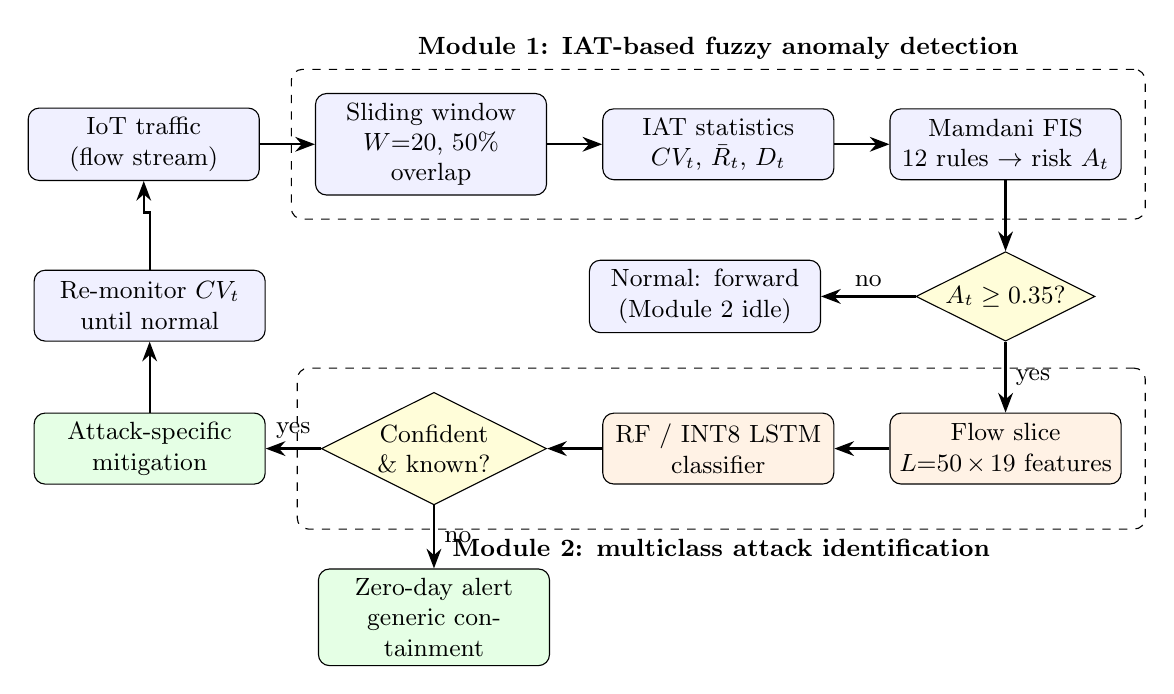
\begin{tikzpicture}[
  node distance=5mm and 7mm,
  box/.style={draw, rounded corners, align=center, minimum height=9mm, text width=27mm, font=\small, fill=blue!6},
  m2/.style={box, fill=orange!10},
  mit/.style={box, fill=green!10},
  dec/.style={draw, diamond, aspect=2, align=center, font=\small, inner sep=1pt, fill=yellow!15},
  arr/.style={-{Stealth[length=2.5mm]}, thick}]
\node[box] (in) {IoT traffic\\(flow stream)};
\node[box, right=of in] (win) {Sliding window\\$W{=}20$, 50\% overlap};
\node[box, right=of win] (feat) {IAT statistics\\$CV_t$, $\bar{R}_t$, $D_t$};
\node[box, right=of feat] (fis) {Mamdani FIS\\12 rules $\rightarrow$ risk $A_t$};
\node[dec, below=9mm of fis] (gate) {$A_t \ge 0.35$?};
\node[box, left=12mm of gate] (pass) {Normal: forward\\(Module 2 idle)};
\node[m2, below=9mm of gate] (seq) {Flow slice\\$L{=}50\times19$ features};
\node[m2, left=of seq] (clf) {RF / INT8 LSTM\\classifier};
\node[dec, left=of clf] (rej) {Confident\\\& known?};
\node[mit, below=8mm of rej] (zd) {Zero-day alert\\generic containment};
\node[mit, left=of rej] (mit) {Attack-specific\\mitigation};
\node[box, above=9mm of mit] (re) {Re-monitor $CV_t$\\until normal};
\begin{scope}[on background layer]
\node[draw, dashed, rounded corners, fit=(win)(feat)(fis), inner sep=3mm, label={[font=\small\bfseries]above:Module 1: IAT-based fuzzy anomaly detection}] {};
\node[draw, dashed, rounded corners, fit=(seq)(clf)(rej), inner sep=3mm, label={[font=\small\bfseries]below:Module 2: multiclass attack identification}] {};
\end{scope}
\draw[arr] (in) -- (win);
\draw[arr] (win) -- (feat);
\draw[arr] (feat) -- (fis);
\draw[arr] (fis) -- (gate);
\draw[arr] (gate) -- node[above,font=\small]{no} (pass);
\draw[arr] (gate) -- node[right,font=\small]{yes} (seq);
\draw[arr] (seq) -- (clf);
\draw[arr] (clf) -- (rej);
\draw[arr] (rej) -- node[above,font=\small]{yes} (mit);
\draw[arr] (rej) -- node[right,font=\small]{no} (zd);
\draw[arr] (mit) -- (re);
\draw[arr] (re.north) |- ($(in.south)+(0,-4mm)$) -- (in.south);
\end{tikzpicture}}
\caption{Architecture of the proposed two-stage IDS. Module~1 screens every window cheaply; Module~2 is only invoked for suspicious or attack windows, and its output drives the attack-specific mitigation and re-monitoring loop.}
\label{fig:arch}
\end{figure}

% ---------------------------------------------------------------------
\subsection{Module 1: IAT-Based Anomaly Detection}
% ---------------------------------------------------------------------

\subsubsection{Packet inter-arrival time}
The IAT of the $i$-th packet is the time between its arrival and the arrival of the previous packet:
\begin{equation}
  \mathrm{IAT}_i = t_i - t_{i-1},
  \label{eq:iat}
\end{equation}
where $t_i$ is the arrival timestamp of packet $i$. In a live deployment, Eq.~\eqref{eq:iat} is computed directly at the gateway. The public CSV release of CICIoT2023 does not provide packet timestamps but does provide an \texttt{IAT} feature extracted by the capture tool. We use this feature directly and do not synthesise or back-calculate timestamps, so the evaluation does not depend on fabricated timing.

\subsubsection{Overlapping sliding windows}
The observation stream is divided into windows of $W$ consecutive records with step $S=W(1-\rho)$, where $\rho$ is the overlap. We use $W=20$ and $\rho=0.5$ ($S=10$), so window $t$ covers records $[tS,\,tS+W-1]$. Each window's ground truth is derived from its attack fraction,
\begin{equation}
  \phi_t = \frac{1}{W}\sum_{i\in t}\mathbf{1}\!\left(y_i \neq \texttt{BenignTraffic}\right),\qquad
  Y_t = \mathbf{1}(\phi_t \ge 0.5),
\end{equation}
and the dominant class label is kept for cohort-level analysis.

\subsubsection{Window-level statistical features}
For each window we compute the mean and standard deviation of IAT,
\begin{equation}
  \mu_t = \frac{1}{W}\sum_{i=1}^{W}\mathrm{IAT}_i, \qquad
  \sigma_t = \sqrt{\frac{1}{W}\sum_{i=1}^{W}\left(\mathrm{IAT}_i-\mu_t\right)^2},
\end{equation}
and the dimensionless coefficient of variation
\begin{equation}
  CV_t = \frac{\sigma_t}{\mu_t + \epsilon}, \qquad \epsilon = 10^{-12}.
  \label{eq:cv}
\end{equation}
Two further features add volumetric and baseline-relative information: the mean packet rate $\bar{R}_t = \frac{1}{W}\sum_i \mathrm{Rate}_i$, and the relative IAT deviation from the clean normal baseline,
\begin{equation}
  D_t = \frac{\left|\mu_t - \mu_{\mathrm{N}}\right|}{\mu_{\mathrm{N}}},
  \label{eq:dev}
\end{equation}
where $\mu_{\mathrm{N}}$ is the mean IAT of benign training traffic only. Benign IoT traffic shows Poisson-like jitter with $CV\approx1$. Automated floods emit packets at a near-constant clock, so $CV\to0$. Scans and probes produce irregular sweeps, so $CV$ and $D$ are large. Figures~\ref{fig:iat}--\ref{fig:rate} show these distributions in the data.

\begin{figure}[t]
\centering
\subfigure[IAT distribution]{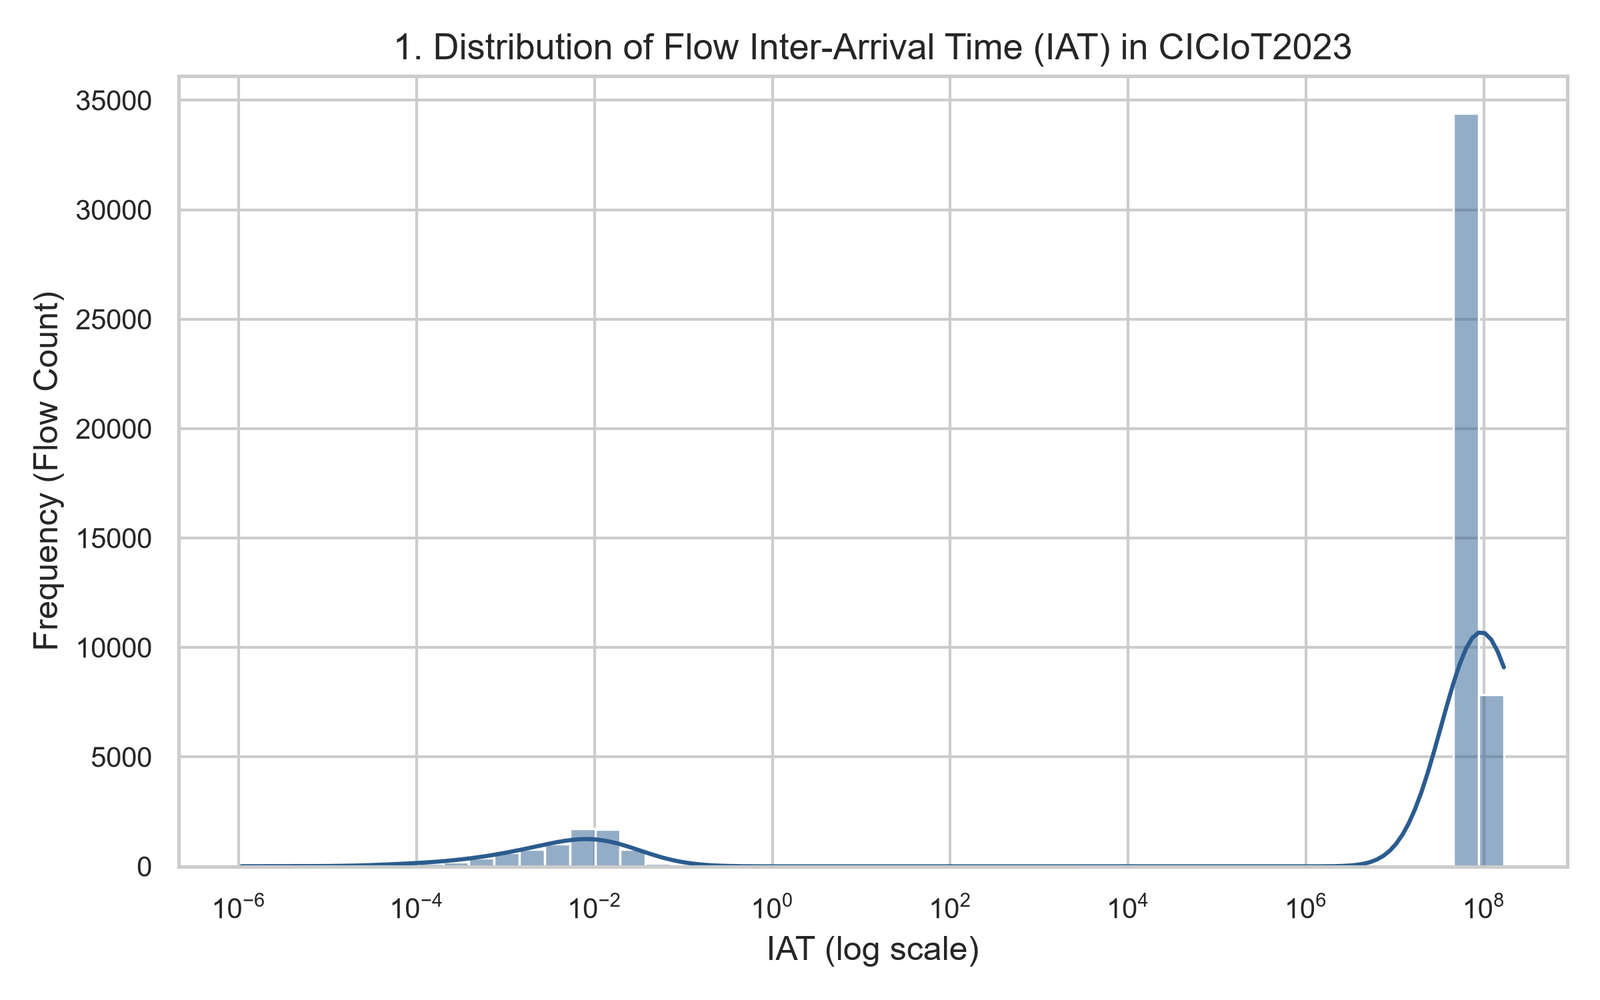
\includegraphics[width=0.48\textwidth]{01_iat_distribution.png}}\hfill
\subfigure[IAT: normal vs.\ attack]{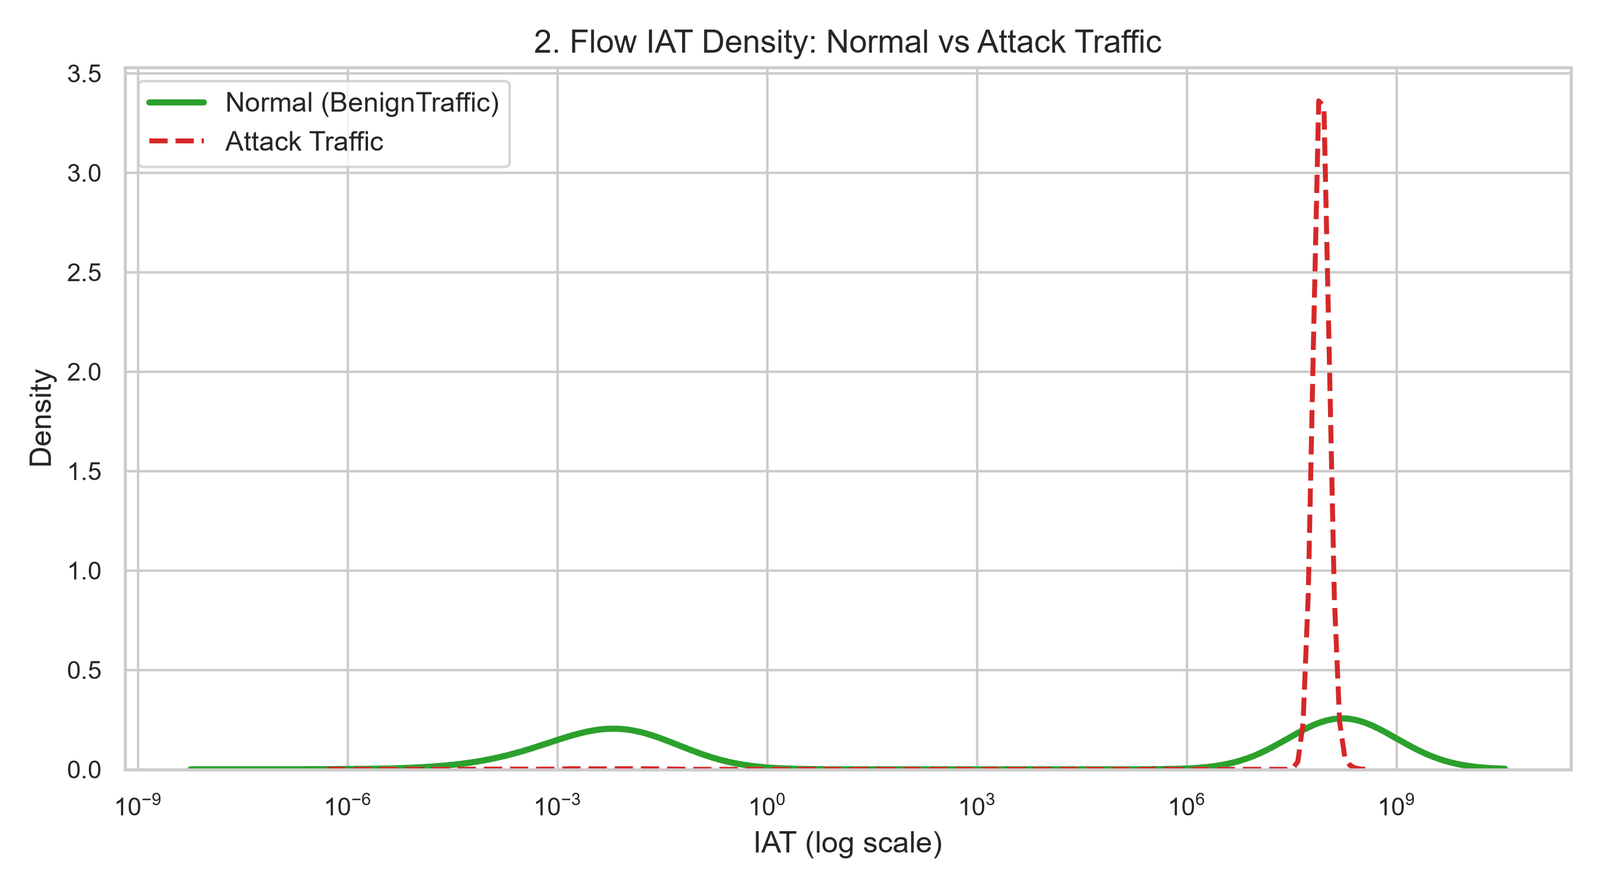
\includegraphics[width=0.48\textwidth]{02_iat_normal_vs_attack.png}}
\caption{Distribution of the packet inter-arrival time feature in CICIoT2023 and its separation between benign and attack traffic.}
\label{fig:iat}
\end{figure}

\begin{figure}[t]
\centering
\subfigure[Window CV of IAT]{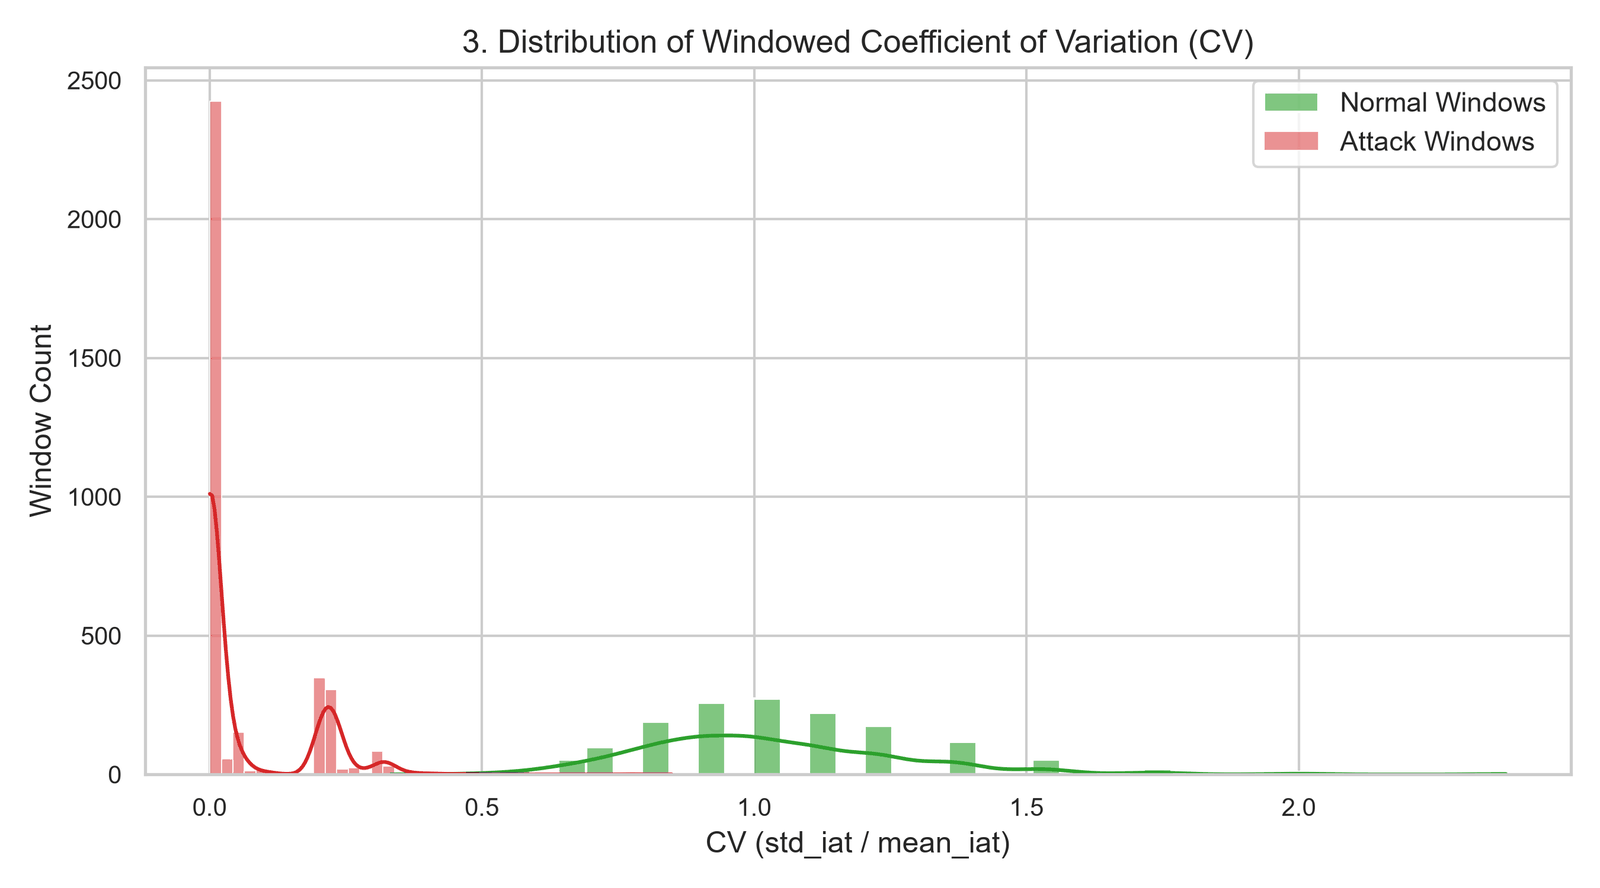
\includegraphics[width=0.48\textwidth]{03_cv_distribution.png}}\hfill
\subfigure[Window mean packet rate]{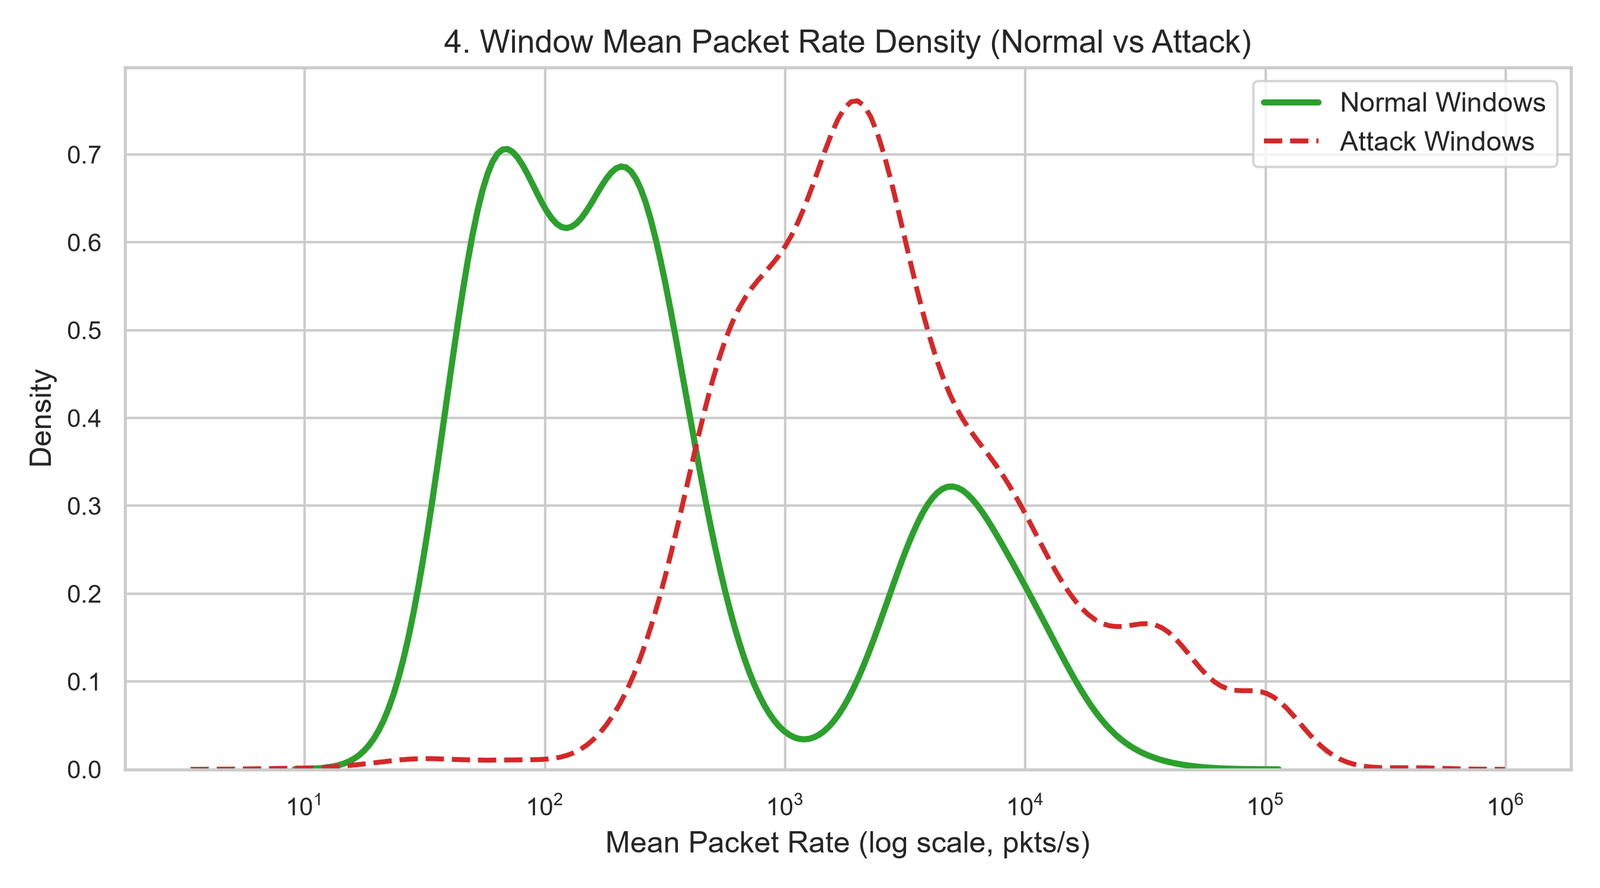
\includegraphics[width=0.48\textwidth]{04_packet_rate_distribution.png}}
\caption{Window-level CV and packet-rate distributions. Many attack windows have CV values below the benign mode. Upper-tail CV tests cannot detect these windows.}
\label{fig:rate}
\end{figure}

\subsubsection{Adaptive Median+MAD threshold with anti-poisoning}
An adaptive threshold is computed from a history $H_t$ of CV values taken from previously accepted normal windows:
\begin{align}
  M_t &= \operatorname{Median}(H_t), \\
  \mathrm{MAD}_t &= \operatorname{Median}\left(\left|CV_j - M_t\right| : CV_j \in H_t\right), \\
  T_t &= M_t + k\cdot \mathrm{MAD}_t ,
  \label{eq:thr}
\end{align}
with sensitivity $k=3$ and a bounded history buffer of 500 windows. If the history is updated with every window, as in a naive adaptive threshold, attack windows are absorbed into $H_t$, the threshold widens and the detector gradually becomes blind (baseline poisoning). We therefore update the history only when the window is confidently normal:
\begin{equation}
  H_{t+1} = \begin{cases} H_t \cup \{CV_t\}, & CV_t \le T_t \ \wedge\ A_t < 0.35,\\ H_t, & \text{otherwise,}\end{cases}
\end{equation}
where $A_t$ is the fuzzy attack risk defined below. Figure~\ref{fig:thr} shows the CV timeline and the adaptive threshold.

\begin{figure}[t]
\centering
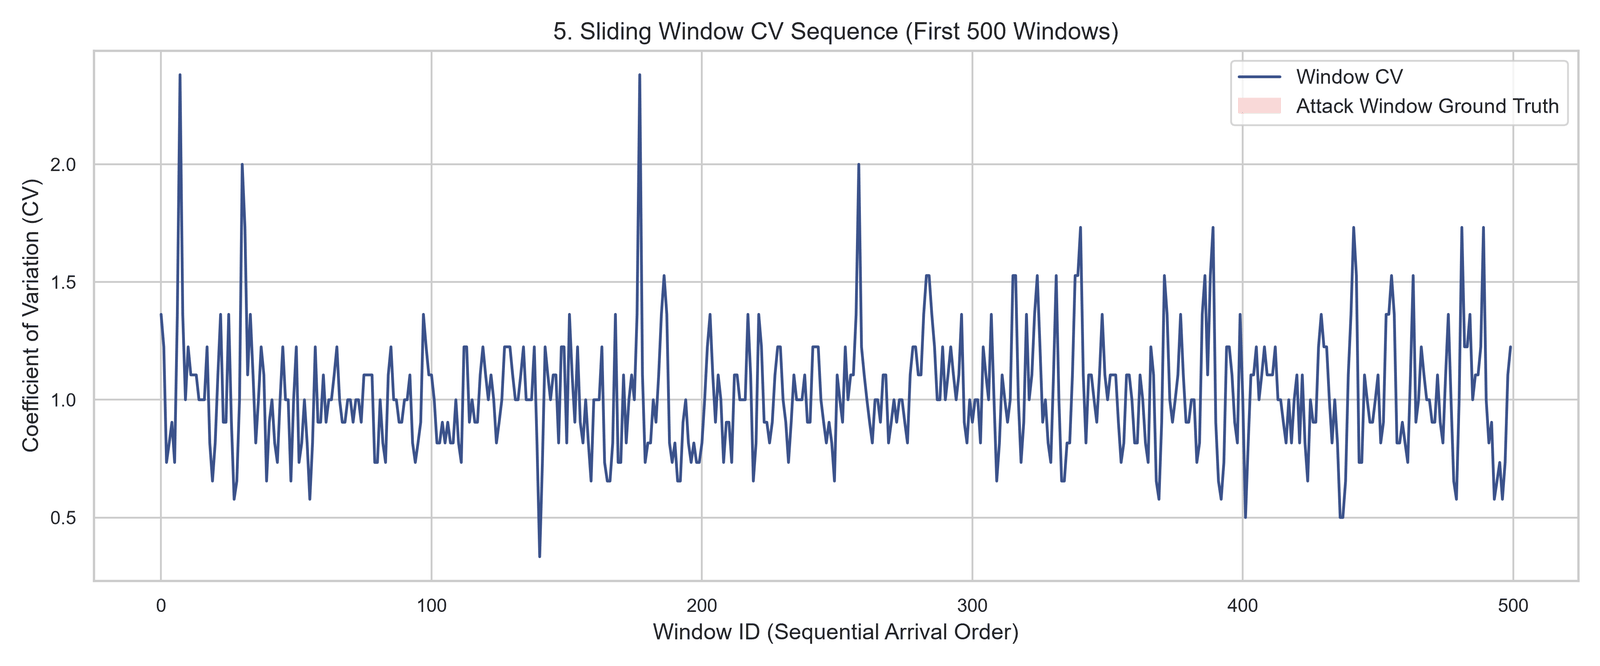
\includegraphics[width=\textwidth]{05_sliding_window_cv_timeline.png}\\[2mm]
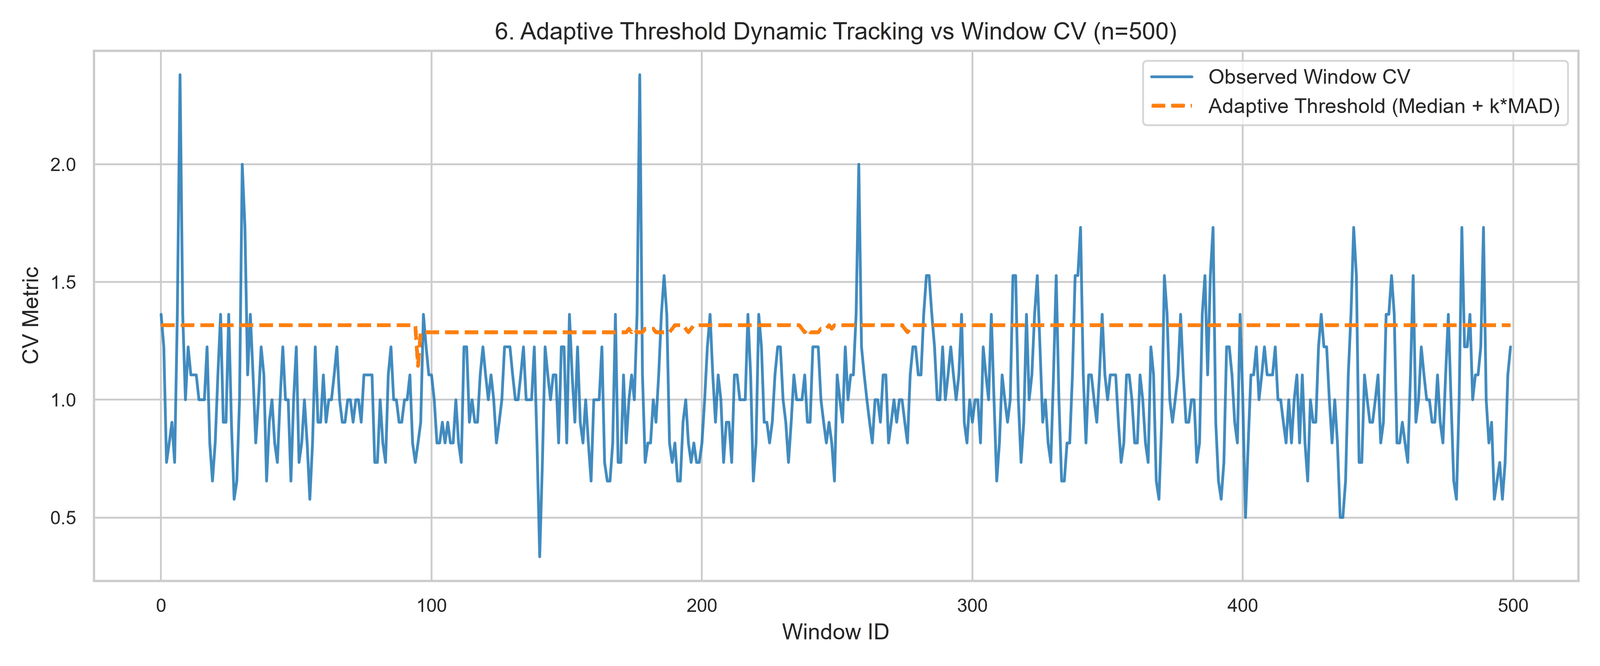
\includegraphics[width=\textwidth]{06_adaptive_threshold_vs_cv.png}
\caption{Top: sliding-window $CV_t$ over the evaluation stream. Bottom: the adaptive Median+MAD threshold $T_t$ against $CV_t$. Flood phases push $CV_t$ well below the threshold, so a CV-only upper-tail test misses them.}
\label{fig:thr}
\end{figure}

\subsubsection{Mamdani fuzzy inference}
Thresholding a single statistic cannot capture anomalies in both directions. We therefore fuse three inputs, $CV_t$, $\bar{R}_t$ and $D_t$, in a Mamdani fuzzy inference system (FIS):
\begin{equation}
  A_t = f_{\mathrm{FIS}}\left(CV_t,\ \bar{R}_t,\ D_t\right) \in [0,1].
\end{equation}
Each input has three linguistic terms (LOW, MEDIUM, HIGH) with triangular or trapezoidal membership functions. Their boundaries are set from percentiles of the clean benign baseline, not chosen by hand (Table~\ref{tab:mf}, Figure~\ref{fig:mf}). For example, the benign CV median is 1.00 with MAD 0.106, its 25th--75th percentile range is 0.82--1.11, and the benign median packet rate is 202\,pkt/s.

\begin{table}[t]
\tbl{Data-driven membership functions of the Mamdani FIS.}
{\begin{tabular}{llll}
\toprule
Variable & LOW & MEDIUM & HIGH \\
\midrule
$CV_t$ (0--6)            & trimf(0, 0, 0.65) & trimf(0.50, 1.02, 1.55) & trapmf(1.40, 1.80, 6, 6) \\
$\bar{R}_t$ (pkt/s)      & trimf(0, 0, 350) & trimf(200, 600, 1500) & trapmf(1000, 2500, 5$\times10^4$, 5$\times10^4$) \\
$D_t$ (0--5)             & trimf(0, 0, 0.18) & trimf(0.12, 0.35, 0.65) & trapmf(0.50, 0.90, 5, 5) \\
Risk $A_t$ (0--1)        & trimf(0, 0, 0.35) & trimf(0.25, 0.50, 0.75) & trapmf(0.60, 0.85, 1, 1) \\
\bottomrule
\end{tabular}}
\label{tab:mf}
\end{table}

\begin{figure}[t]
\centering
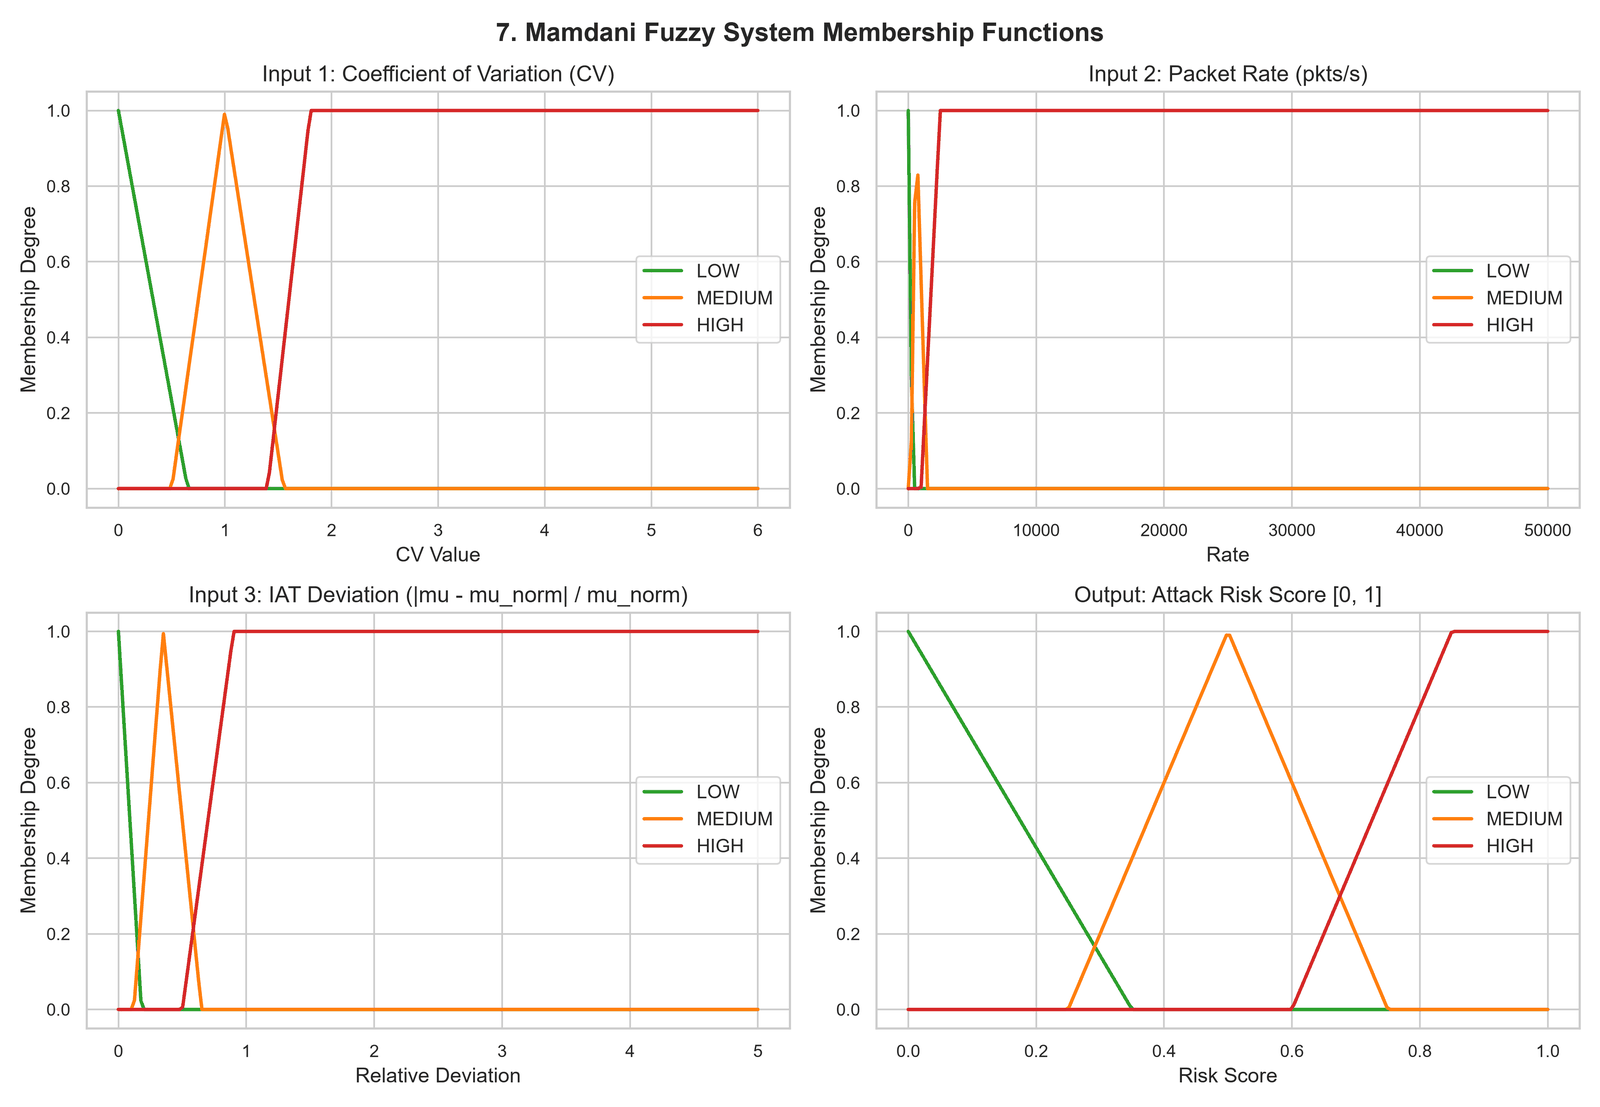
\includegraphics[width=0.9\textwidth]{07_fuzzy_membership_functions.png}
\caption{Membership functions of the three antecedents (CV, packet rate, IAT deviation) and the attack-risk consequent.}
\label{fig:mf}
\end{figure}

The rule base (Table~\ref{tab:rules}) encodes domain knowledge. Rule R11 (LOW CV $\wedge$ HIGH rate $\Rightarrow$ HIGH risk) captures constant-rate floods such as DoS and Mirai, and rule R12 captures stealthy, low-rate scans. Rules are combined with min (AND) and max (aggregation) operators.

\begin{table}[t]
\tbl{Interpretable fuzzy rule base.}
{\begin{tabular}{clcl}
\toprule
Rule & Antecedent & Risk & Rationale \\
\midrule
R1  & CV MED $\wedge$ Rate LOW $\wedge$ Dev LOW  & LOW  & Steady-state IoT behaviour \\
R2  & CV LOW $\wedge$ Rate LOW $\wedge$ Dev LOW  & LOW  & Periodic low-rate beaconing \\
R3  & CV HIGH $\wedge$ Rate HIGH                 & HIGH & Volumetric burst DDoS \\
R4  & CV HIGH $\wedge$ Dev HIGH                  & HIGH & Pulse attack / recon sweep \\
R5  & Rate HIGH $\wedge$ Dev HIGH                & HIGH & Volumetric attack with timing shift \\
R6  & CV MED $\wedge$ Rate HIGH                  & HIGH & High-rate Poisson-like flood \\
R7  & CV HIGH $\wedge$ Rate MED                  & HIGH & Irregular burst attack \\
R8  & CV MED $\wedge$ Rate MED $\wedge$ Dev MED  & MED  & Borderline activity \\
R9  & Rate HIGH                                  & HIGH & Volumetric override \\
R10 & Dev HIGH                                   & HIGH & Timing-channel collapse \\
R11 & CV LOW $\wedge$ Rate HIGH                  & HIGH & Constant-rate flood (DoS/Mirai) \\
R12 & CV HIGH $\wedge$ Rate LOW                  & MED  & Stealthy scan / slow probe \\
\bottomrule
\end{tabular}}
\label{tab:rules}
\end{table}

\subsubsection{Defuzzification and decision}
The aggregated output fuzzy set is defuzzified with the centroid method,
\begin{equation}
  A_t = \frac{\int z\,\mu_{\mathrm{agg}}(z)\,dz}{\int \mu_{\mathrm{agg}}(z)\,dz},
\end{equation}
and mapped to three decision zones:
\begin{equation}
  \text{Verdict}_t = \begin{cases}
  \textsc{Normal}, & A_t < 0.35,\\
  \textsc{Suspicious}, & 0.35 \le A_t < 0.65,\\
  \textsc{Attack}, & A_t \ge 0.65.
  \end{cases}
\end{equation}
Windows labelled \textsc{Suspicious} or \textsc{Attack} are forwarded to Module~2. \textsc{Normal} windows are released without further processing.

% ---------------------------------------------------------------------
\subsection{Module 2: Multiclass Attack Identification}
% ---------------------------------------------------------------------

\subsubsection{Traffic buffering and feature selection}
Module~1 uses only timing and rate statistics, so extracting the full feature set for every window would waste resources. A ring buffer holds the most recent flow records. When Module~1 flags window $t$, the slice of $L=50$ consecutive flows ending at that window is retrieved. Each flow is described by 19 features chosen from the 46 available in CICIoT2023 (Table~\ref{tab:feat}). Labels, scenario identifiers and IP addresses are excluded to prevent leakage and protect privacy.

\begin{table}[t]
\tbl{Features used by Module 2.}
{\begin{tabular}{lp{0.62\textwidth}}
\toprule
Group & Features \\
\midrule
Timing \& rate     & IAT, Rate, Srate, Drate, flow\_duration, Duration \\
Volume \& size     & Header\_Length, Tot size, Tot sum, Number, AVG, Std, Min, Max \\
Protocol \& state  & Protocol Type, TCP, UDP, syn\_count, ack\_count \\
\bottomrule
\end{tabular}}
\label{tab:feat}
\end{table}

\subsubsection{Leakage-safe preprocessing and sequence construction}
Missing values are imputed with training-set medians, infinite values are clipped to the finite training maximum, and a \texttt{StandardScaler} fitted on training flows only is applied to every split. A provenance audit showed that the Kaggle CSVs are row-shuffled, so arbitrary consecutive rows mix unrelated classes. Sequences are therefore built only inside homogeneous class blocks, and the train/validation/test split (70/15/15) is made on the blocks \emph{before} sequences are formed. This ensures that overlapping sequences never cross the split boundary. Sequences have shape $(L,F)=(50,19)$, with step 25 for training and 15 for evaluation.

\subsubsection{Classifiers}
\textbf{LSTM.} An \texttt{LSTM(64)} layer is followed by \texttt{Dropout(0.2)}, \texttt{Dense(32, ReLU)} and a 31-way softmax. It is trained with Adam (learning rate $10^{-3}$, batch 64) and sparse categorical cross-entropy, with early stopping (patience 5). The recurrence is statically unrolled over the 50 time steps to remove dynamic \texttt{TensorList} operations, which allows native full-integer TFLite conversion.

\textbf{Random Forest baseline.} A pure-NumPy Random Forest (30 trees, maximum depth 12, percentile split candidates) uses non-sequential inputs: the last observation of the sequence plus the per-feature mean and standard deviation over the sequence. It shows whether recurrent modelling adds value over simple aggregates.

\subsubsection{INT8 post-training quantisation}
The FP32 LSTM is converted to a full-integer INT8 TFLite model with a representative calibration set drawn from the training sequences. For a tensor with observed range $[r_{\min}, r_{\max}]$, affine quantisation uses
\begin{gather}
  s = \frac{r_{\max}-r_{\min}}{q_{\max}-q_{\min}}, \qquad
  z = \operatorname{round}\!\left(q_{\min} - \frac{r_{\min}}{s}\right), \\
  q = \operatorname{clip}\!\left(\operatorname{round}\!\left(\frac{r}{s}\right) + z,\ q_{\min},\ q_{\max}\right),
\end{gather}
with $q_{\min}=-128$ and $q_{\max}=127$, and dequantisation $\hat{r}=s(q-z)$. Inference runs on the XNNPACK CPU delegate.

\subsubsection{Zero-day rejection}
A closed-set classifier always outputs one of its known classes. To flag unknown traffic, we apply maximum-softmax-probability (MSP) rejection,
\begin{equation}
  \hat{Y}_t = \begin{cases}
  \arg\max_k p_k, & \max_k p_k \ge \tau,\\
  \textsc{Unknown (zero-day)}, & \text{otherwise},
  \end{cases}
\end{equation}
with $\tau=0.0643$ set to the 10th percentile of the confidence of correct validation predictions.

% ---------------------------------------------------------------------
\subsection{Attack-Specific Mitigation and Re-Monitoring}
% ---------------------------------------------------------------------
The identified class $\hat{Y}_t$ selects a mitigation action according to the attack family (Table~\ref{tab:mitig}). Unknown traffic receives a conservative containment action and an operator alert. After an action is applied, Module~1 keeps computing $CV_t$, $\bar{R}_t$ and $D_t$. Mitigation is considered successful when the fuzzy risk falls back below 0.35 for a run of consecutive windows. Otherwise the response is escalated, for example from rate limiting to blocking. In the current prototype, this mapping is implemented as a decision policy in the dashboard; enforcing actions in the network data plane is left for future work.

\begin{table}[t]
\tbl{Attack-family to mitigation mapping.}
{\begin{tabular}{lp{0.58\textwidth}}
\toprule
Identified family & Mitigation action \\
\midrule
DDoS / DoS floods        & Per-source rate limiting, SYN cookies, upstream traffic filtering / blackholing \\
Botnet (Mirai-like)      & Quarantine infected device, block C\&C endpoints, enforce credential reset \\
Reconnaissance / scans   & Temporary source block, port-scan throttling, honeypot redirection \\
Spoofing / MITM          & Dynamic ARP inspection, static ARP bindings, DNSSEC validation \\
Web / brute force        & Account lockout, CAPTCHA/back-off, WAF signature update \\
Unknown (zero-day)       & Rate-limit and isolate segment, capture traffic, raise operator alert \\
\bottomrule
\end{tabular}}
\label{tab:mitig}
\end{table}

% =====================================================================
\section{Dataset and Experimental Setup}\label{sec:setup}
% =====================================================================

\subsection{CICIoT2023 dataset}
CICIoT2023 is a large-scale IoT benchmark captured from a topology of 105 IoT devices. We use its public CSV release, which contains 6{,}668{,}822 flows across 34 classes: \texttt{BenignTraffic} plus DDoS and DoS floods, the Mirai botnet family, reconnaissance and vulnerability scans, spoofing/MITM, and web/application attacks (SQL injection, command injection, XSS, browser hijacking, dictionary brute force, back-door malware and uploading attacks).

\subsection{Zero-day protocol}
All three Mirai classes (\texttt{Mirai-\allowbreak greeth\_\allowbreak flood}, \texttt{Mirai-\allowbreak greip\_\allowbreak flood} and \texttt{Mirai-\allowbreak udpplain}) are held out as a zero-day proxy. They are excluded from the benign baseline, the membership-function boundaries, the threshold calibration, the scaler and label encoder, and classifier training, and are introduced only in the final test stream. Module~2 therefore covers 31 known classes. Holding out an entire family is an empirical proxy for novel attacks, not a guarantee against all future exploits.

\subsection{Evaluation stream and metrics}
Module~1 is evaluated on a phased stream of 50{,}000 flows, which gives 4{,}999 windows: 1{,}499 normal, 2{,}499 known-attack and 999 held-out Mirai windows. Three detectors are compared on the same stream: (i) a \emph{simple CV threshold} (flag if $CV_t$ exceeds the 95th percentile of benign CV); (ii) the \emph{adaptive Median+MAD} threshold with anti-poisoning; and (iii) the proposed \emph{fuzzy} system, where a window counts as detected when $A_t \ge 0.35$. We report accuracy, precision, recall (TPR), F1-score and false-positive rate (FPR). Module~2 is evaluated on held-out test sequences with accuracy, macro-F1, weighted-F1, mean and P95 CPU latency per sequence, and model size. All experiments use random seed 42 and run on a desktop Intel Core i7 CPU with Python, scikit-fuzzy and TensorFlow/TFLite.

% =====================================================================
\section{Results and Discussion}\label{sec:results}
% =====================================================================

\subsection{Anomaly detection performance (Module 1)}

Table~\ref{tab:m1} and Figure~\ref{fig:cm} compare the three detectors. The simple CV threshold detects no attack windows (recall 0\%), and the adaptive MAD threshold reaches only 3.51\% recall. Both methods test the upper tail ($CV_t > T$), but the dominant flood attacks in CICIoT2023 \emph{lower} IAT dispersion (often $CV\approx0.002$), so these windows fall below any upper threshold. The fuzzy system fuses dispersion, rate and baseline deviation and reaches 82.24\% accuracy, 85.69\% precision, 89.60\% recall and 87.60\% F1. Its main cost is a 34.98\% false-positive rate, mostly from bursty benign windows assigned to the \textsc{Suspicious} band. These windows are not dropped: they are passed to Module~2 for verification.

\begin{table}[t]
\tbl{Anomaly detection performance on 4{,}999 windows.}
{\begin{tabular}{lcccccc}
\toprule
Method & Accuracy & Precision & Recall & F1-score & FPR & Mirai det. \\
\midrule
Simple CV threshold   & 28.49\% & 0.00\%  & 0.00\%  & 0.00\%  & \textbf{4.94}\% & 0.00\% \\
Adaptive Median+MAD   & 29.35\% & 44.40\% & 3.51\%  & 6.51\%  & 10.28\% & 11.61\% \\
\textbf{Fuzzy (proposed)} & \textbf{82.24\%} & \textbf{85.69\%} & \textbf{89.60\%} & \textbf{87.60\%} & 34.98\% & \textbf{75.88\%} \\
\bottomrule
\end{tabular}}
\label{tab:m1}
\end{table}

\begin{figure}[t]
\centering
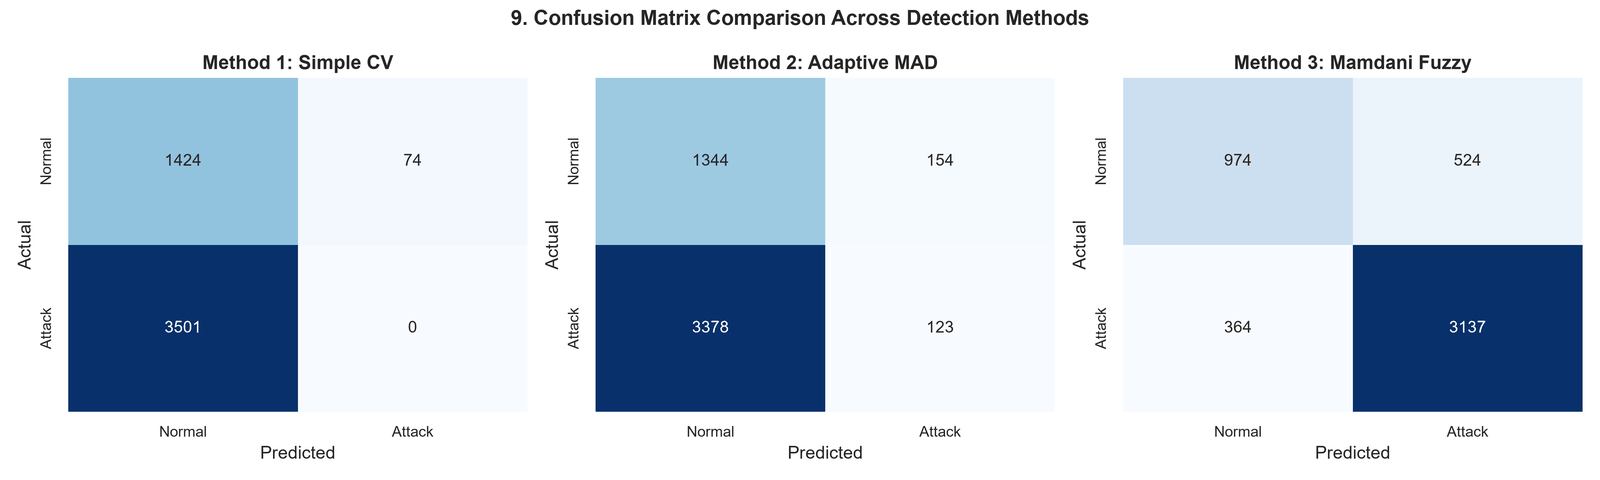
\includegraphics[width=\textwidth]{09_confusion_matrices.png}
\caption{Window-level confusion matrices of the simple CV, adaptive MAD and fuzzy detectors (TN/FP/FN/TP of 1424/74/3501/0, 1344/154/3378/123 and 974/524/364/3137 respectively).}
\label{fig:cm}
\end{figure}

\begin{figure}[t]
\centering
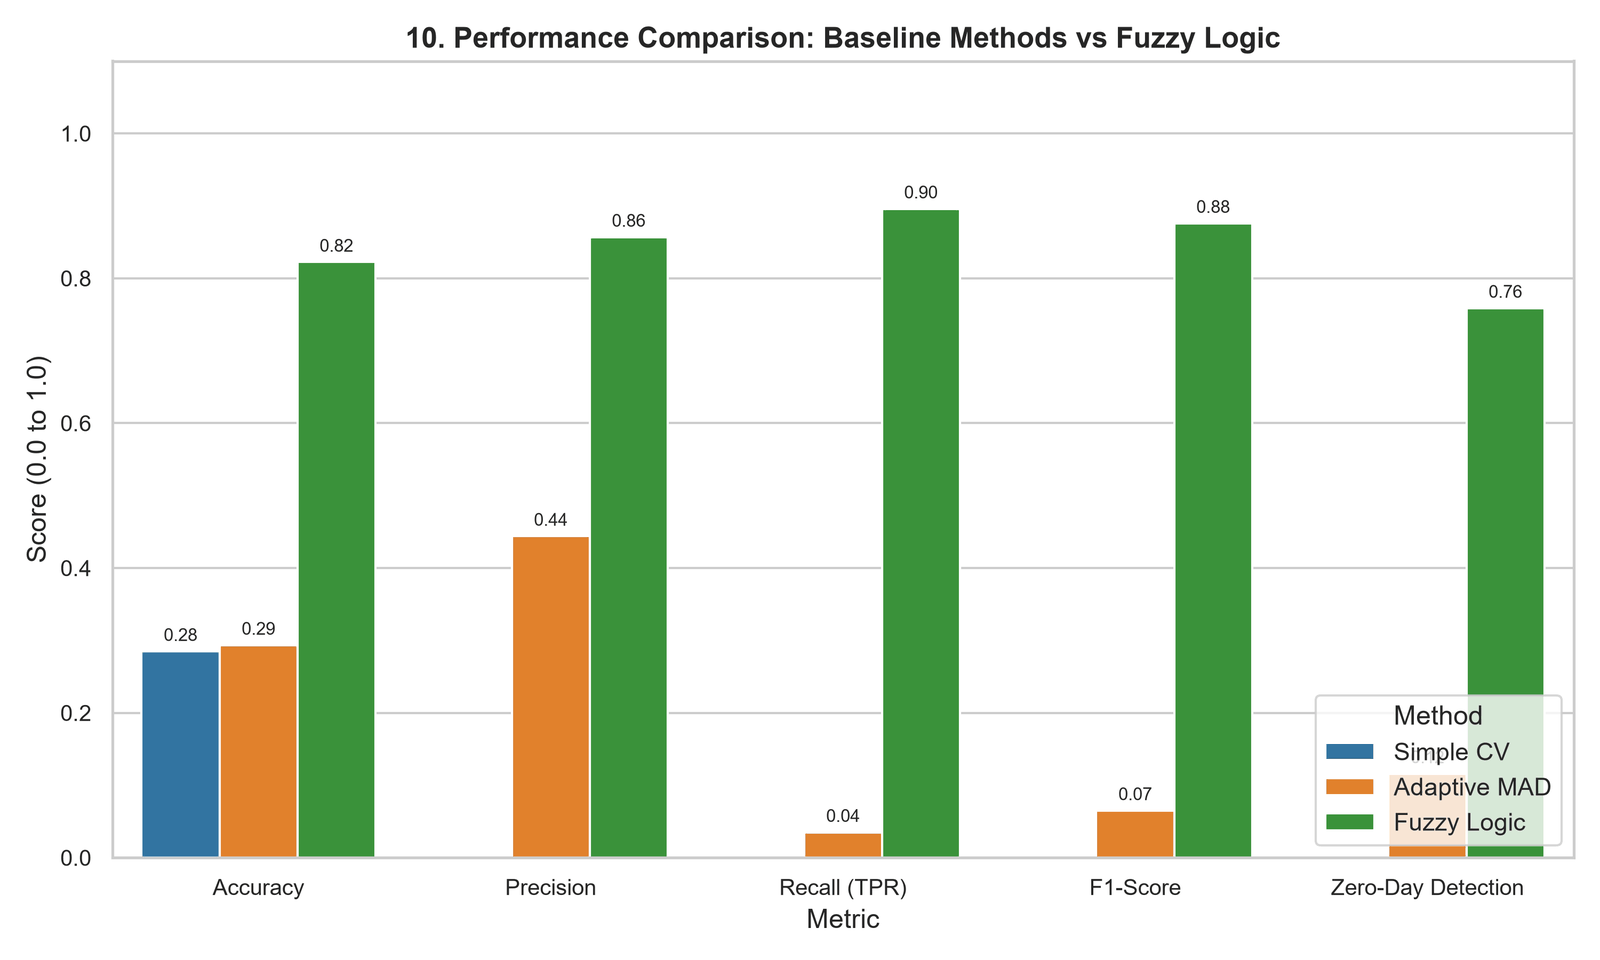
\includegraphics[width=0.75\textwidth]{10_performance_comparison.png}
\caption{Accuracy, precision, recall, F1 and FPR of the three anomaly detectors.}
\label{fig:perf}
\end{figure}

Table~\ref{tab:cohort} breaks the alarm rate down by cohort. The fuzzy detector flags 95.08\% of known-attack windows and 75.88\% of held-out Mirai windows, against 0\% and 11.61\% for the best threshold baseline. The mean fuzzy risk is 0.37 for normal windows, 0.79 for known attacks and 0.59 for unseen Mirai traffic. The risk timeline in Figure~\ref{fig:risk} shows that the score rises clearly when attack phases begin.

\begin{table}[t]
\tbl{Alarm rate per traffic cohort.}
{\begin{tabular}{lcccc}
\toprule
Cohort (windows) & Simple CV & Adaptive MAD & Fuzzy & Mean risk $A_t$ \\
\midrule
Normal (1{,}499)          & 4.94\% & 13.54\% & 34.96\% & 0.374 $\pm$ 0.290 \\
Known attacks (2{,}499)   & 0.00\% & 15.73\% & \textbf{95.08\%} & 0.792 $\pm$ 0.162 \\
Held-out Mirai (999)      & 0.00\% & 11.61\% & \textbf{75.88\%} & 0.595 $\pm$ 0.278 \\
\bottomrule
\end{tabular}}
\label{tab:cohort}
\end{table}

\begin{figure}[t]
\centering
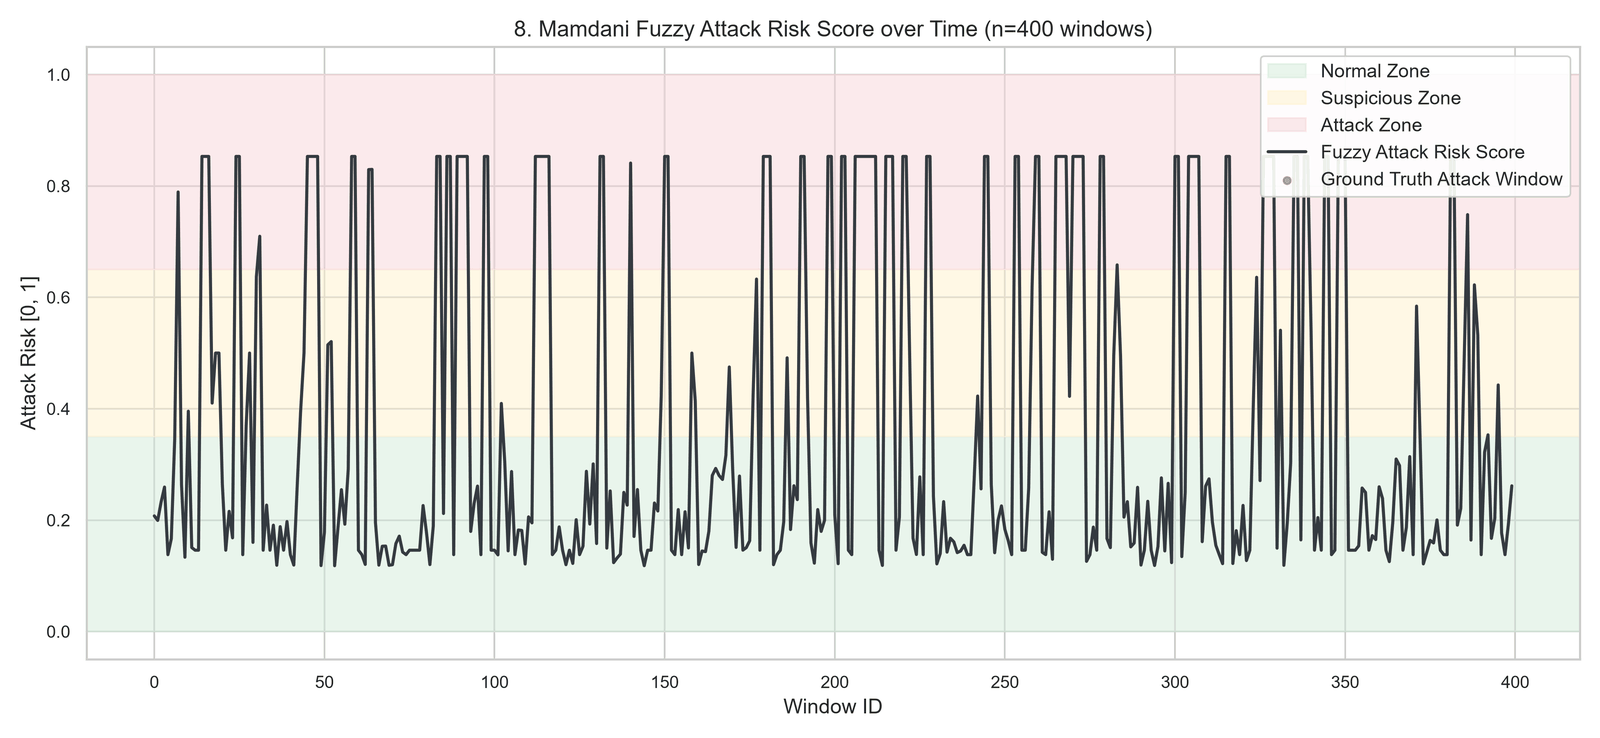
\includegraphics[width=\textwidth]{08_attack_risk_timeline.png}
\caption{Continuous fuzzy attack-risk score over the evaluation stream with the 0.35 and 0.65 decision boundaries.}
\label{fig:risk}
\end{figure}

\paragraph{Sensitivity analysis.}
Figure~\ref{fig:sens} varies the window size and the MAD multiplier. Accuracy peaks at $W=20$ (0.823), compared with 0.727 at $W=10$, 0.807 at $W=50$ and 0.750 at $W=100$. Small windows are noisy, and large windows blur the boundaries between attack phases and delay alerts. For the adaptive MAD baseline, a larger $k$ lowers accuracy steadily (0.280 at $k=2$ to 0.177 at $k=4$), which confirms that tuning $k$ cannot fix its one-sided test.

\begin{figure}[t]
\centering
\subfigure[Window size $W$]{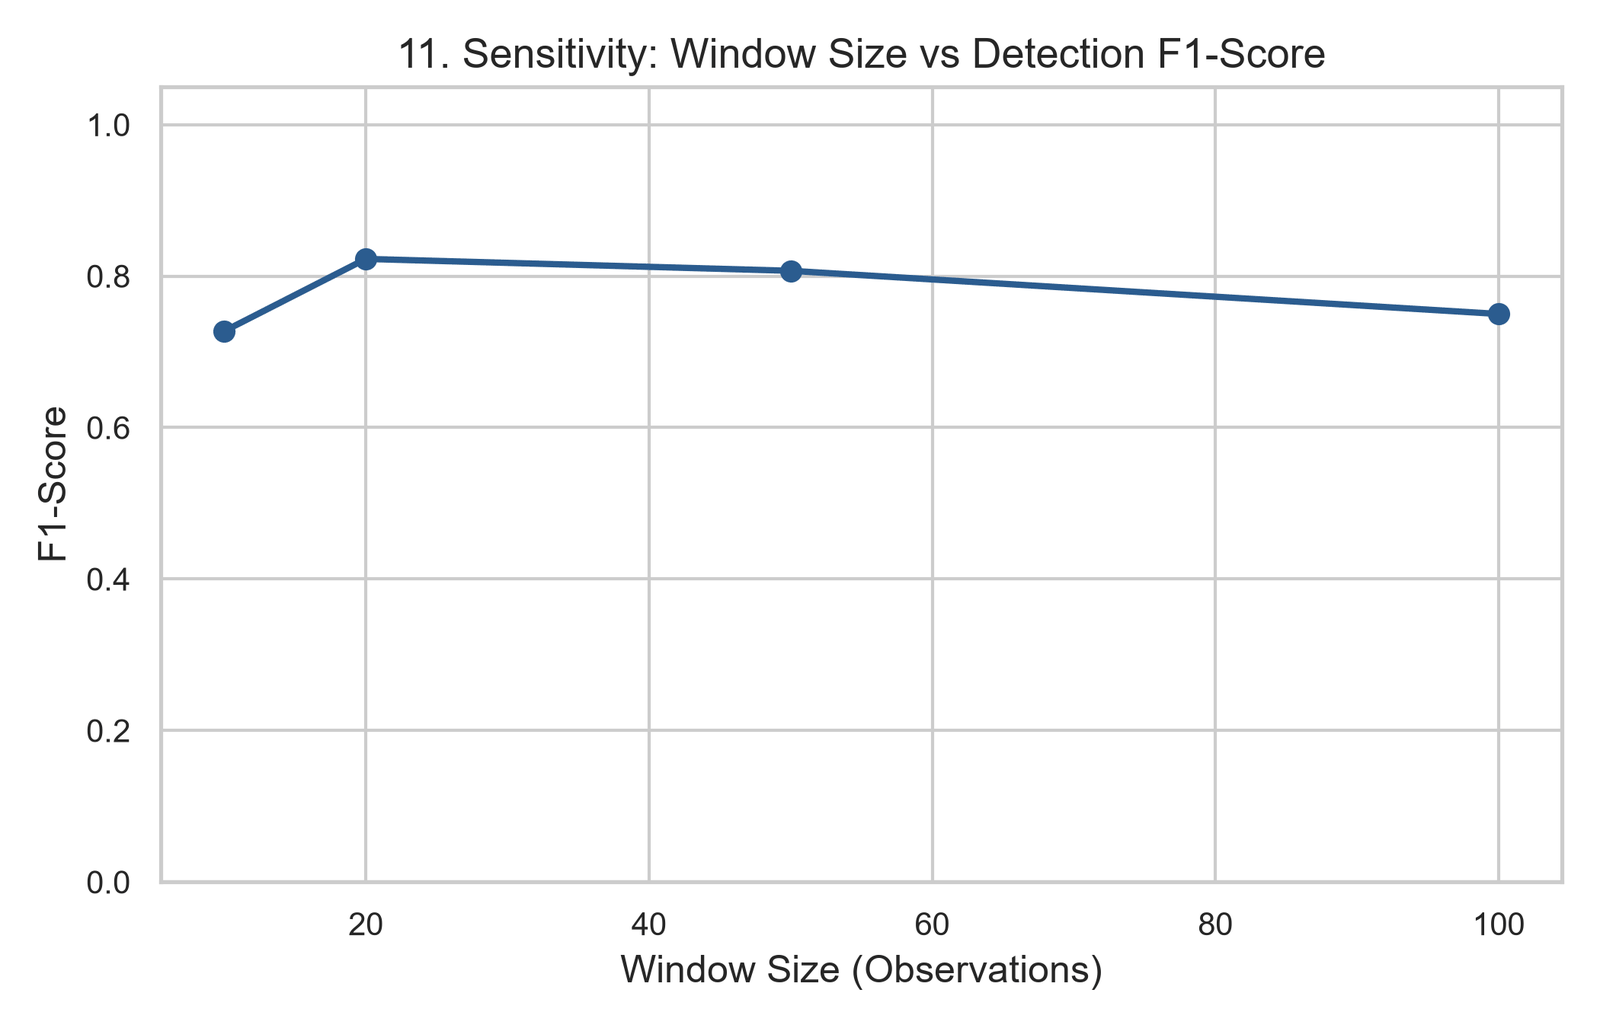
\includegraphics[width=0.48\textwidth]{11_window_size_sensitivity.png}}\hfill
\subfigure[MAD multiplier $k$]{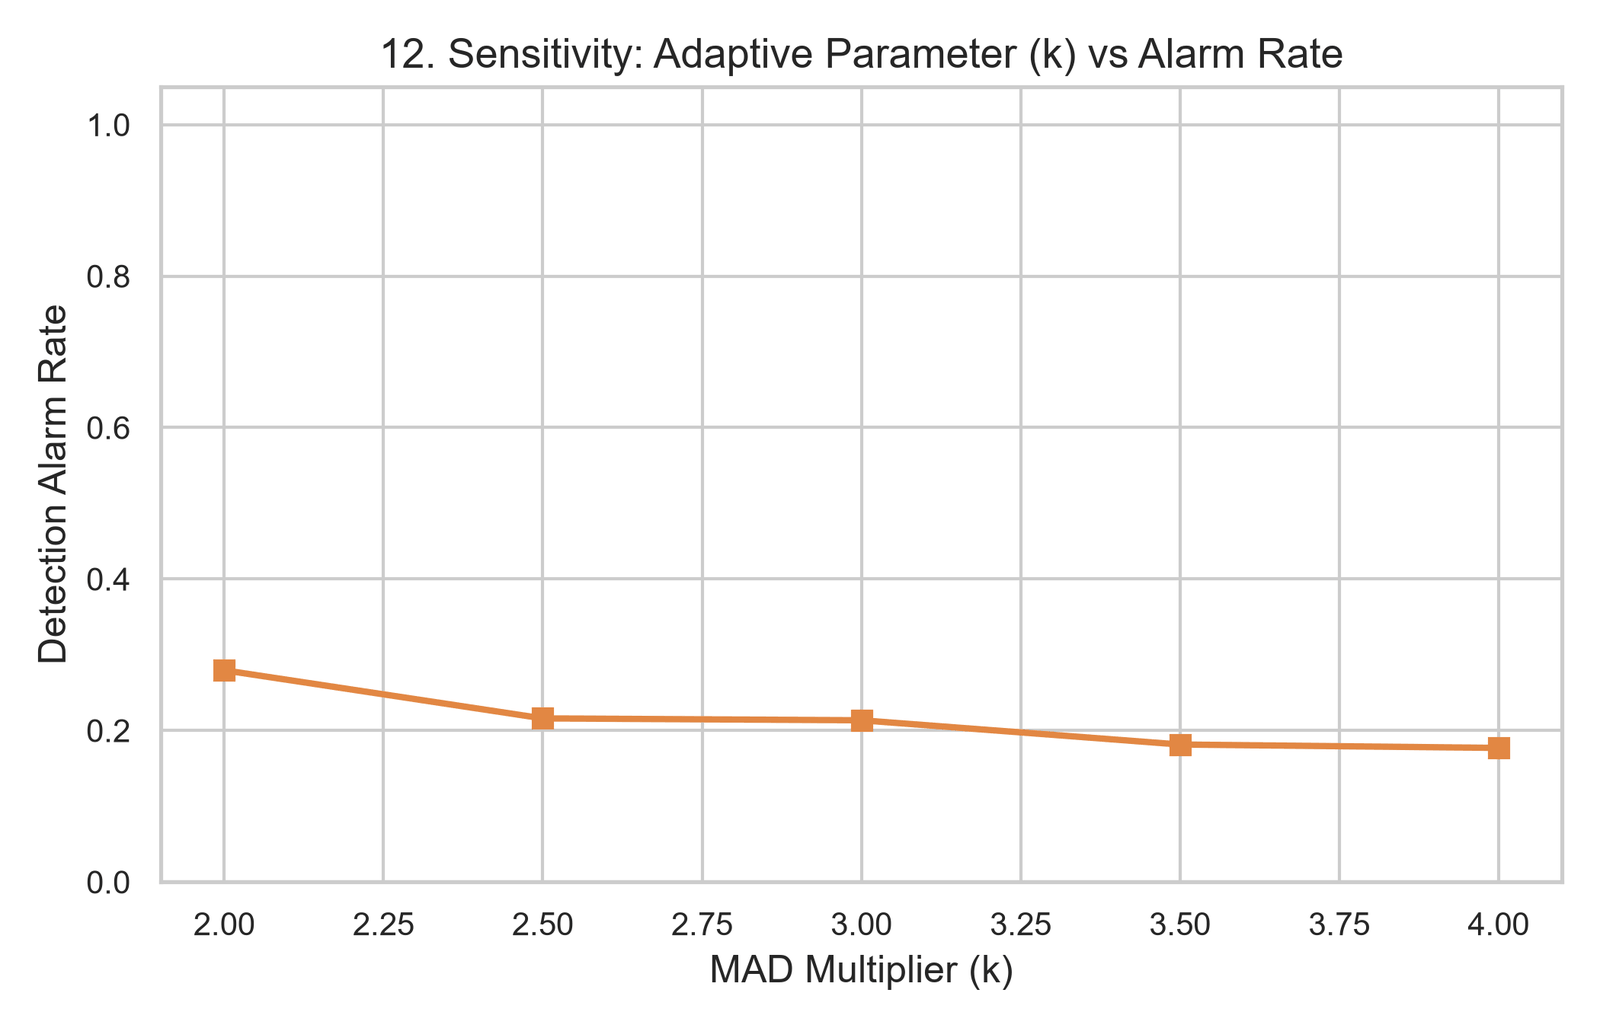
\includegraphics[width=0.48\textwidth]{12_mad_k_sensitivity.png}}
\caption{Sensitivity of detection performance to the sliding-window size and to the adaptive-threshold multiplier.}
\label{fig:sens}
\end{figure}

\subsection{Multiclass classification performance (Module 2)}

Table~\ref{tab:m2} and Figure~\ref{fig:m2cmp} compare the classifiers on 87 held-out test sequences covering the 31 known classes. The Random Forest performs best, with 94.25\% accuracy, 91.77\% macro-F1 and 93.02\% weighted-F1, and perfect per-class F1 on most flood, spoofing and web classes. Its weakest classes are \texttt{Recon-OSScan} (F1 0.50), \texttt{Recon-PortScan} (0.57) and \texttt{DDoS-UDP\_Flood} (0.57), along with the very rare \texttt{Recon-PingSweep} and \texttt{Backdoor\_Malware}, which have only one test sequence each. The compact LSTM reaches only 34.48\% accuracy under the small training budget used here (429 training sequences, a few epochs; Figure~\ref{fig:loss}). Flow-level volumetric aggregates are thus already highly discriminative on CICIoT2023, and the recurrent model needs considerably more data and training to learn temporal transitions across 31 classes.

\begin{table}[t]
\tbl{Multiclass attack identification on the known-class test set.}
{\begin{tabular}{lccccccc}
\toprule
Model & Acc. & Macro-F1 & Wtd-F1 & Lat. mean (ms) & Lat. P95 (ms) & Size (MB) \\
\midrule
Random Forest        & \textbf{94.25\%} & \textbf{91.77\%} & \textbf{93.02\%} & 0.196 & 0.230 & 2.68 \\
FP32 LSTM (Keras)    & 34.48\% & 20.47\% & 21.18\% & 51.070 & 55.096 & 0.31 \\
INT8 LSTM (TFLite)   & 34.48\% & 21.73\% & 22.48\% & \textbf{0.087} & \textbf{0.099} & 0.31 \\
\bottomrule
\end{tabular}}
\label{tab:m2}
\end{table}

\begin{figure}[t]
\centering
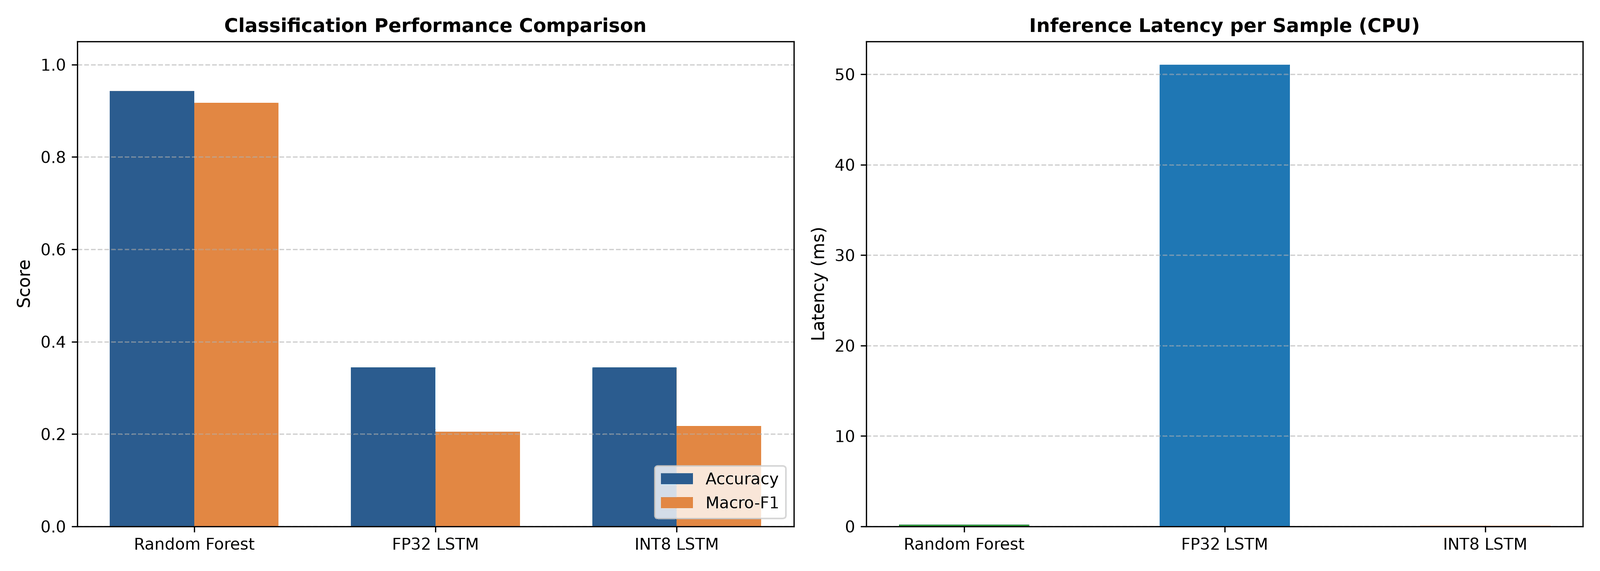
\includegraphics[width=\textwidth]{module2_model_comparison.png}
\caption{Accuracy/F1, latency and model size of the Random Forest, FP32 LSTM and INT8 LSTM.}
\label{fig:m2cmp}
\end{figure}

\begin{figure}[t]
\centering
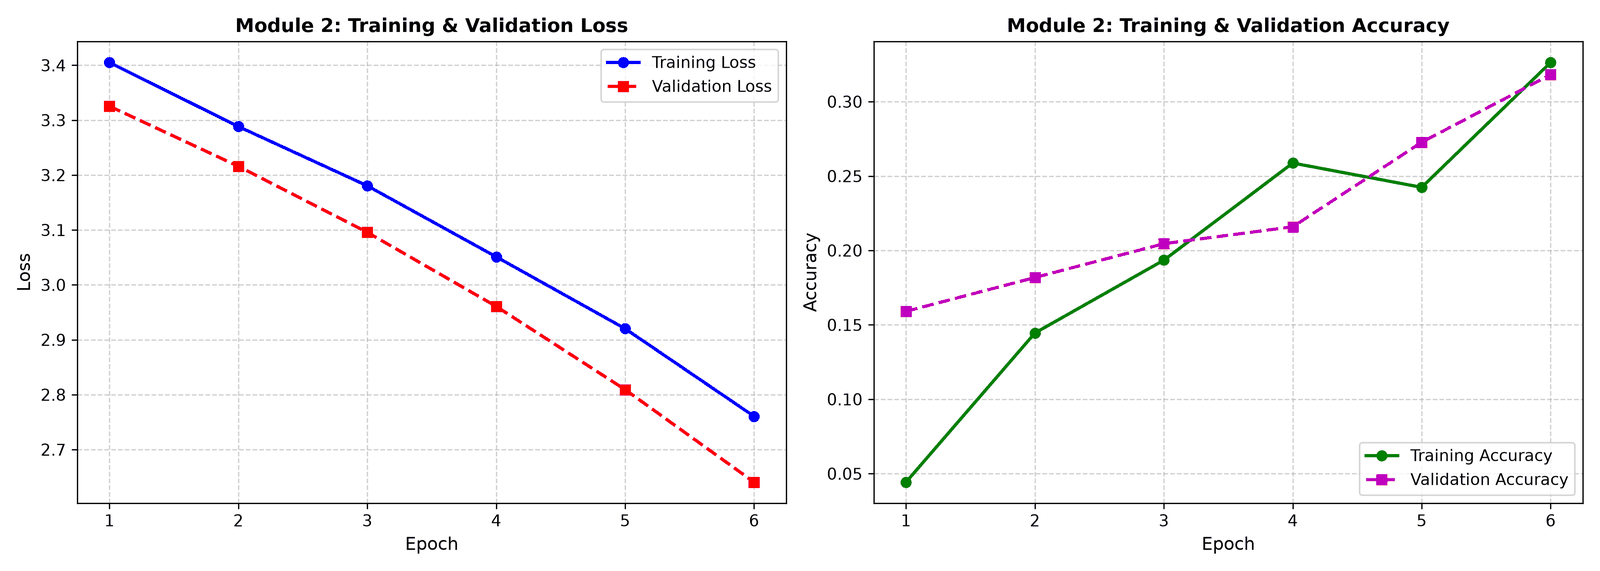
\includegraphics[width=\textwidth]{module2_loss_curves.png}
\caption{Training and validation loss and accuracy of the LSTM.}
\label{fig:loss}
\end{figure}

\begin{figure}[t]
\centering
\subfigure[FP32 LSTM]{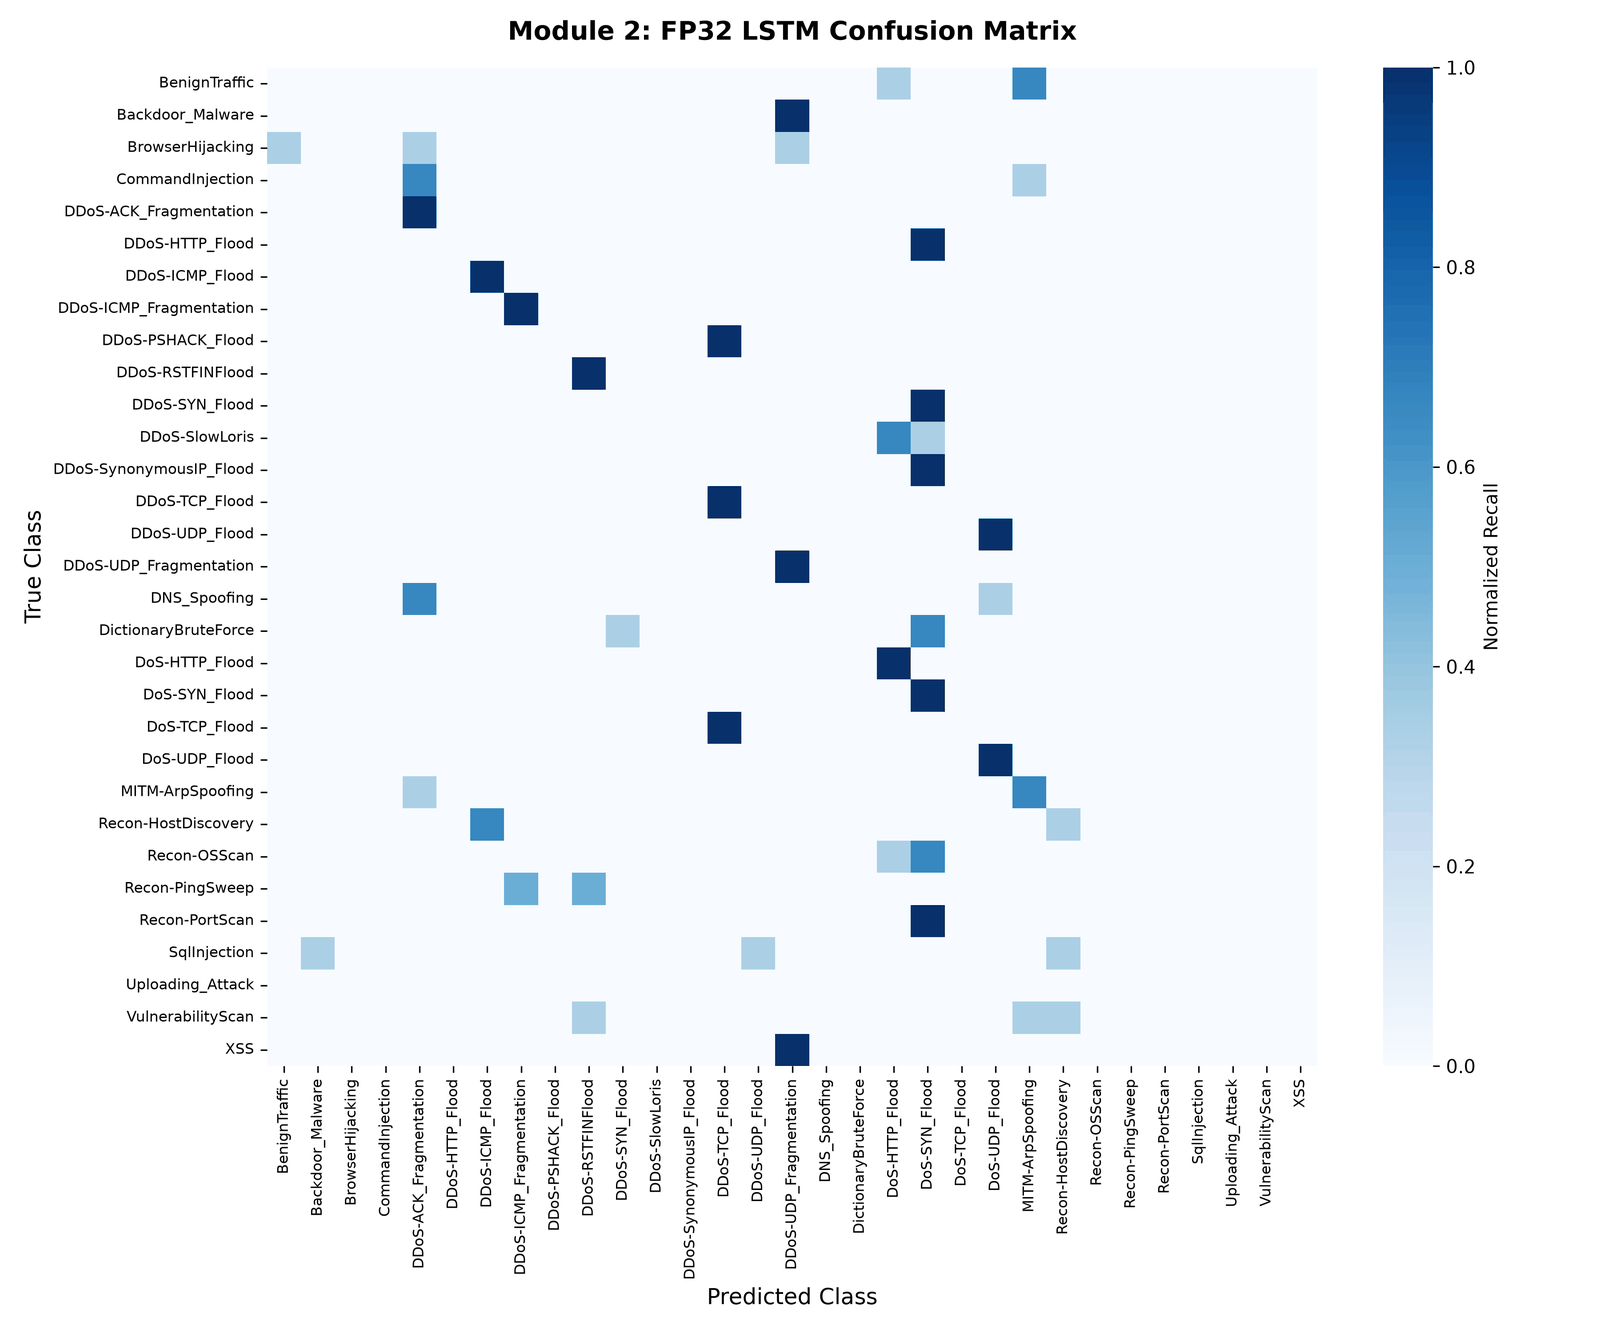
\includegraphics[width=0.48\textwidth]{module2_confusion_matrix_fp32.png}}\hfill
\subfigure[INT8 LSTM]{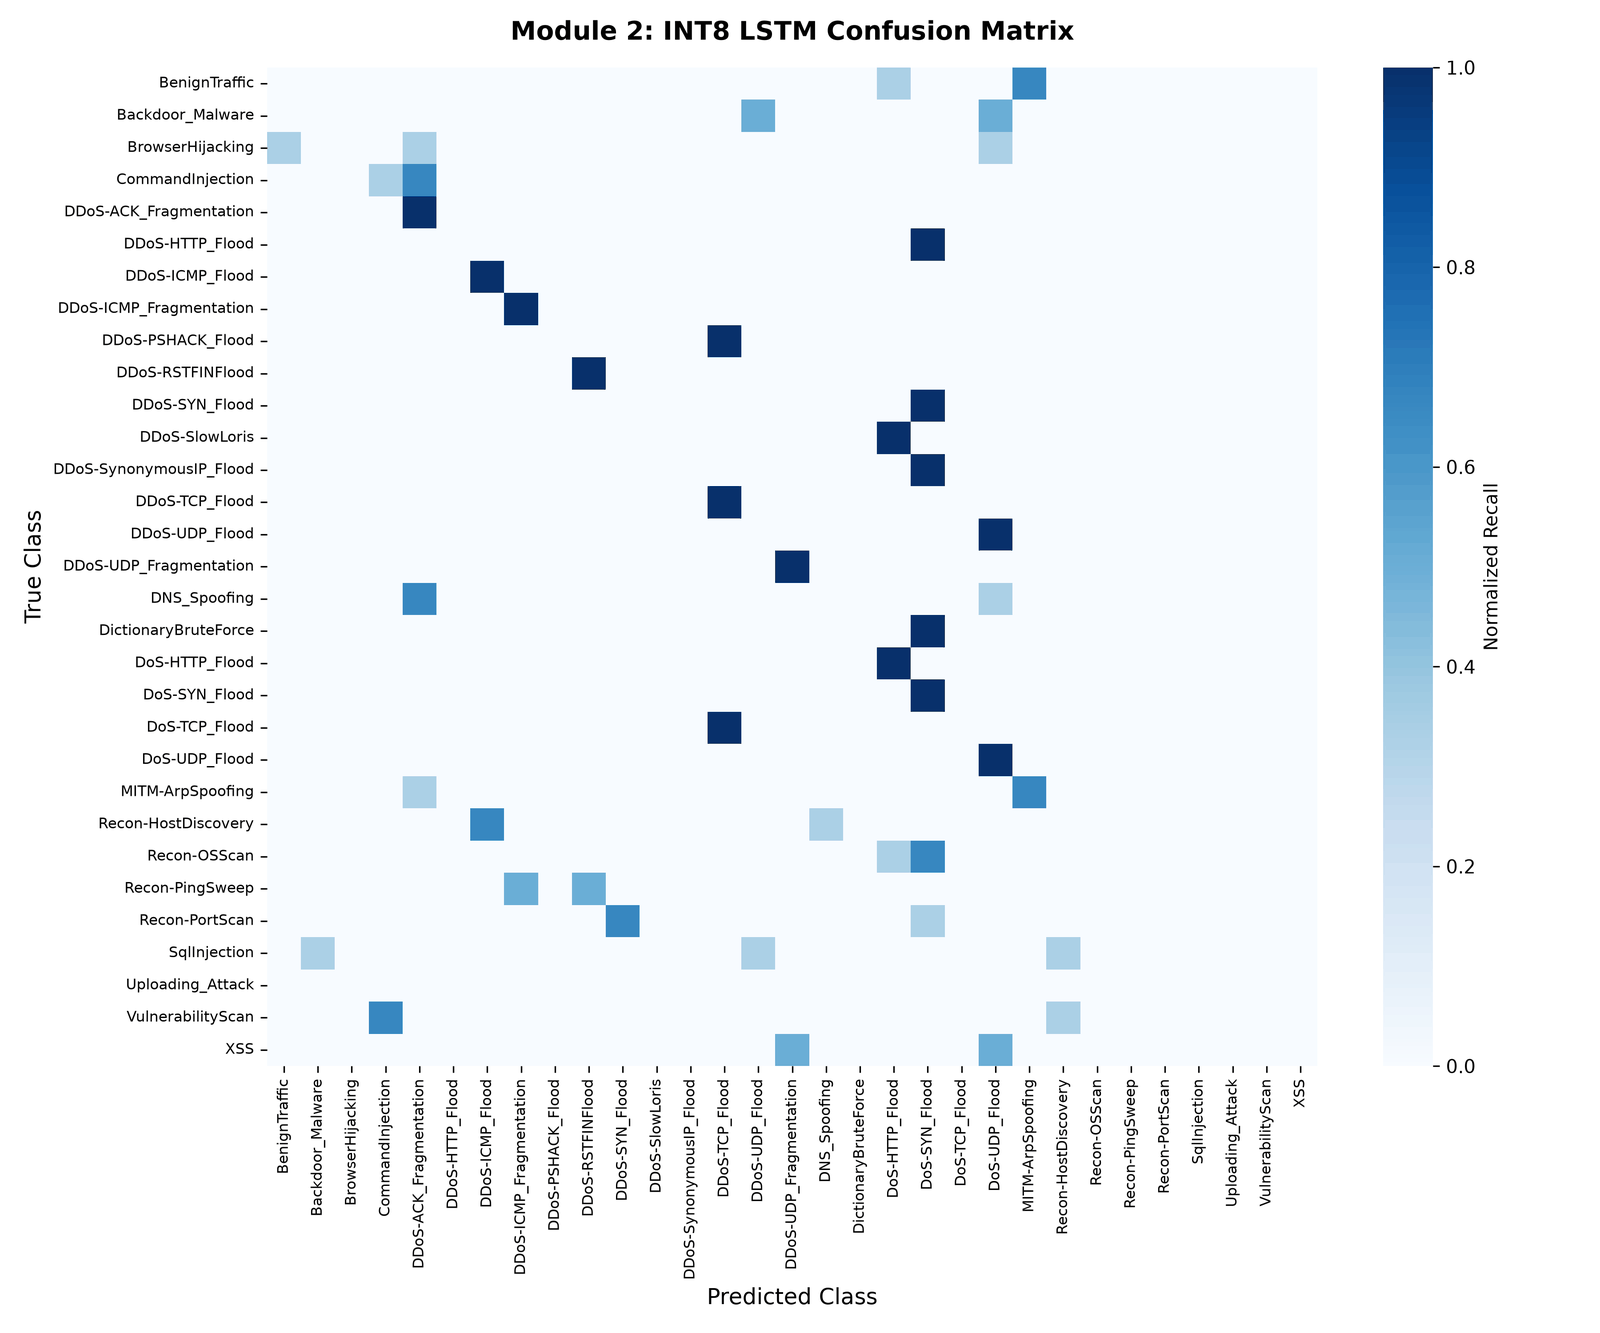
\includegraphics[width=0.48\textwidth]{module2_confusion_matrix_int8.png}}
\caption{Normalised confusion matrices of the LSTM before and after INT8 quantisation.}
\label{fig:m2cm}
\end{figure}

\subsection{Quantisation and computational efficiency}
Full-integer INT8 quantisation keeps the LSTM's accuracy unchanged (34.48\%), slightly raises macro-F1 (20.47\% to 21.73\%) and gives 85.06\% prediction agreement with the FP32 model (Figure~\ref{fig:m2cm}). Mean latency falls from 51.07\,ms to 0.087\,ms per sequence, a speed-up of about $587\times$, and P95 latency falls from 55.10\,ms to 0.099\,ms. Most of this gain comes from replacing the Keras eager runtime with the XNNPACK-accelerated integer TFLite interpreter, not from arithmetic precision alone. The model file size is the same in both formats (0.31\,MB) because the network has few parameters and the file size is dominated by graph structure and metadata. Larger models would show the expected weight-memory reduction of about 75\%.

The two-stage design also saves computation at the system level (Table~\ref{tab:e2e}). Of the 4{,}999 windows, 26.77\% were judged \textsc{Normal} by Module~1 and never reached Module~2, so the classifier ran on only 73.23\% of the windows. The evaluation stream is deliberately attack-heavy. In operational IoT networks, where benign traffic usually dominates, the share of windows that bypass Module~2 would be much larger.

\begin{table}[t]
\tbl{End-to-end gating of Module 2 by Module 1.}
{\begin{tabular}{lccc}
\toprule
Module 1 verdict & Windows & Share & Module 2 invoked \\
\midrule
\textsc{Normal}      & 1{,}338 & 26.77\% & No \\
\textsc{Suspicious}  &   489   &  9.78\% & Yes \\
\textsc{Attack}      & 3{,}172 & 63.45\% & Yes \\
\midrule
Total                & 4{,}999 & 100\%   & 73.23\% \\
\bottomrule
\end{tabular}}
\label{tab:e2e}
\end{table}

\subsection{Held-out (zero-day) attack analysis}\label{sec:zeroday}
The two modules behave very differently on the 111 held-out Mirai sequences. MSP rejection in Module~2 detects none of them (0\% zero-day detection). The unseen Mirai floods receive a \emph{higher} mean confidence (0.202) than known traffic (0.119), and all accepted samples are assigned to similar known classes: 73 to \texttt{DDoS-UDP\_Fragmentation} and 38 to \texttt{DoS-UDP\_Flood}. At the chosen threshold, MSP also wrongly rejects 35.63\% of known traffic. Module~1 does not depend on any attack signature and flags 75.88\% of the Mirai windows because of their abnormal timing and rate. Supervised confidence alone is therefore not a reliable zero-day detector, and the label-free timing filter provides most of the system's zero-day coverage. Combining the two, for example by alerting on windows that Module~1 rates as high-risk but Module~2 assigns with low class-consistency, is a natural extension.

\subsection{Interactive prototype}
The pipeline is also available as an interactive Streamlit dashboard (Figure~\ref{fig:ui}). It lets an analyst enter window statistics or choose attack presets, view the activated fuzzy rules and membership degrees, and see the resulting verdict and recommended mitigation.

\begin{figure}[t]
\centering
\subfigure[Dashboard view]{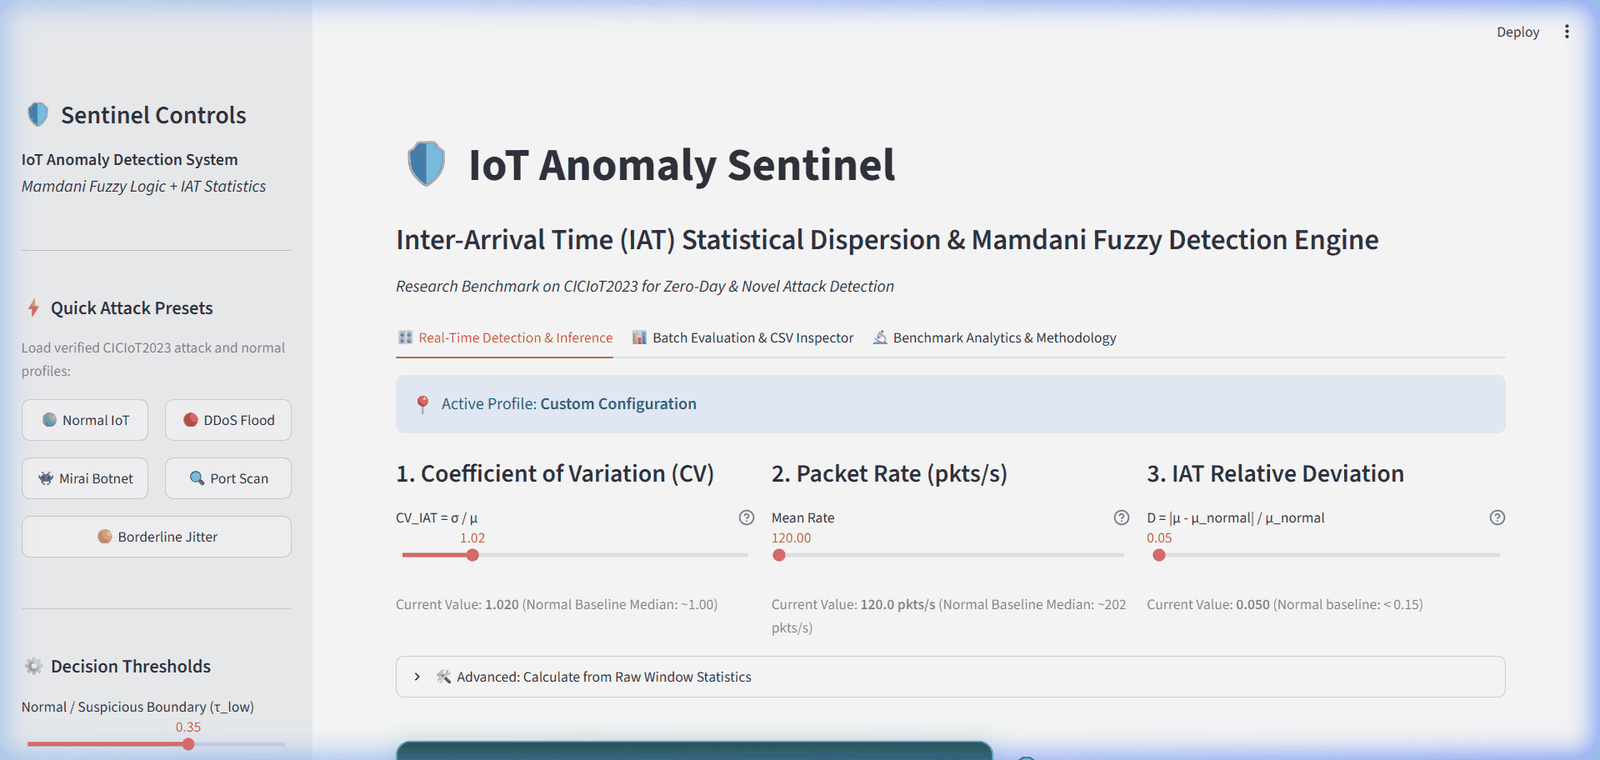
\includegraphics[width=0.48\textwidth]{streamlit_dashboard_view.png}}\hfill
\subfigure[Verdict and rule explanation]{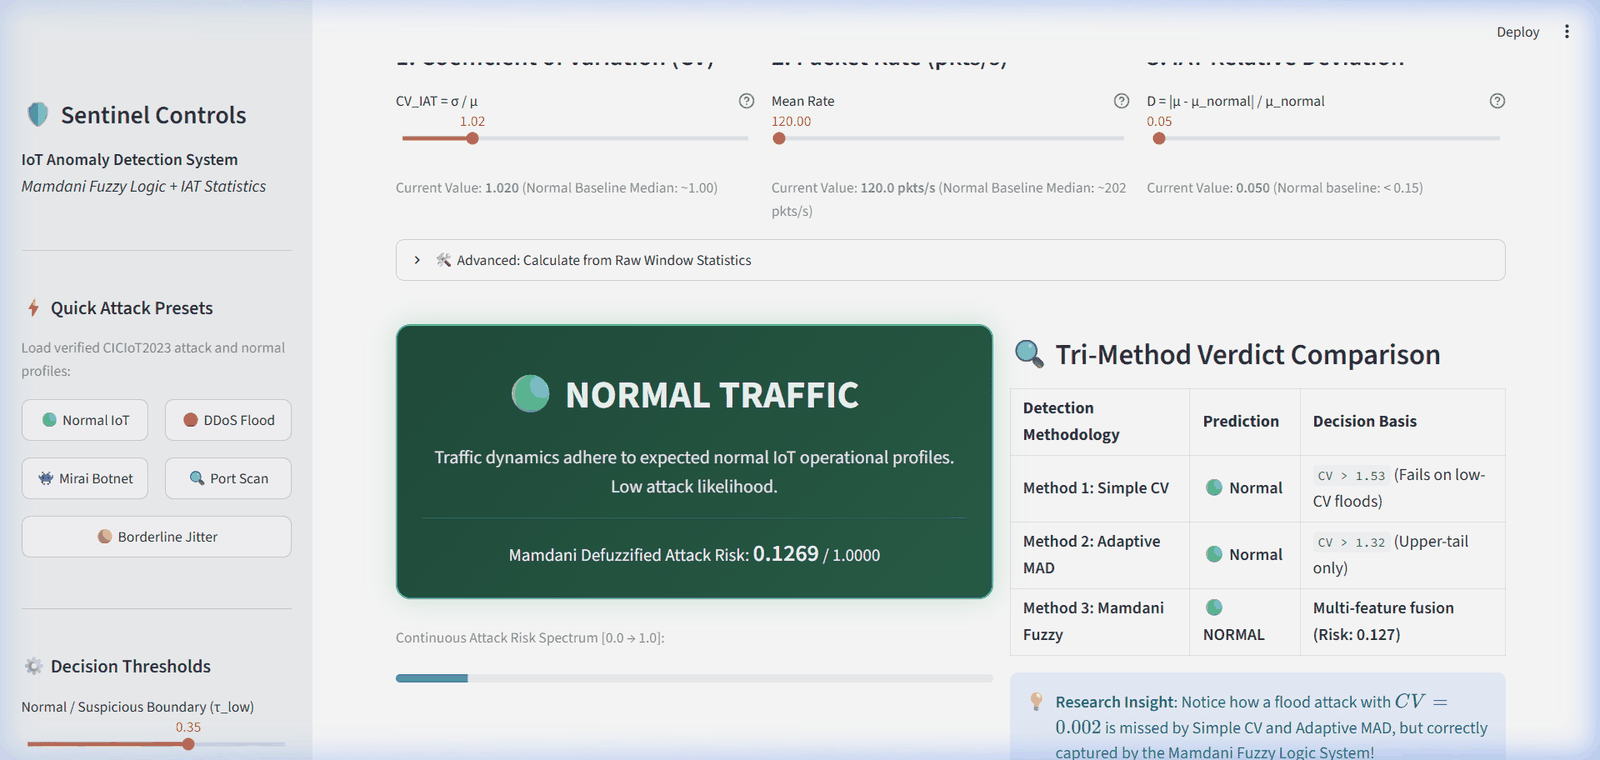
\includegraphics[width=0.48\textwidth]{streamlit_verdict_view.png}}
\caption{Streamlit prototype of the proposed IDS.}
\label{fig:ui}
\end{figure}

% =====================================================================
\section{Limitations}\label{sec:limits}
% =====================================================================
\begin{enumerate}
  \item \textbf{No packet timestamps.} The CSV release of CICIoT2023 omits raw timestamps, so the timing analysis uses the flow-level \texttt{IAT} feature and assumes the record order reflects arrival order. Validation on raw PCAP captures is required.
  \item \textbf{False positives.} The 34.98\% FPR comes mainly from legitimate high-throughput bursts such as firmware updates or streaming. Module~2 verifies these windows, but adding application-layer entropy features or a persistence term to the FIS would reduce the alert load.
  \item \textbf{LSTM training budget.} The LSTM was trained on a small sample budget (600 flows per class), which explains its low accuracy. Its results should be read as a quantisation and latency study rather than as an upper bound on recurrent accuracy.
  \item \textbf{Slow-rate attacks.} Very slow attacks, such as Slowloris with minute-scale gaps, need much longer windows ($W\ge200$) to accumulate enough statistical deviation.
  \item \textbf{Hardware and mitigation.} Latency was measured on a desktop CPU. ARM Cortex-A72 (Raspberry Pi~4) latency is expected to be about 1--3\,ms per sequence but has not yet been measured. The mitigation mapping has not yet been enforced or evaluated in a live testbed.
\end{enumerate}

% =====================================================================
\section{Conclusion and Future Work}\label{sec:conc}
% =====================================================================
This paper presented a lightweight two-stage intrusion detection system for resource-constrained IoT networks. The first stage turns packet inter-arrival time into three interpretable window statistics, the coefficient of variation, the packet rate and the deviation from a clean baseline, and fuses them with a 12-rule Mamdani fuzzy system. On CICIoT2023, the fuzzy detector improves recall from 3.51\% (adaptive MAD) to 89.60\% and F1 from 6.51\% to 87.60\%, mainly because it detects low-dispersion floods that upper-tail CV thresholds cannot, and it flags 75.88\% of a fully held-out Mirai botnet family. The second stage runs only on flagged windows. It identifies 31 known attack classes with 94.25\% accuracy using a compact Random Forest, and INT8 quantisation reduces LSTM inference latency to under 0.1\,ms. The study also shows that softmax-confidence rejection fails completely on unseen Mirai floods, which supports combining a label-free timing filter with supervised attribution.

Future work will (i) replay raw PCAP traces to compute IAT from true packet timestamps; (ii) add a persistence input and adaptive membership functions to reduce false positives; (iii) train the LSTM, or a temporal convolutional network, on the full dataset and use distance-based open-set rejection; (iv) deploy the INT8 pipeline on Raspberry Pi and ESP32-class gateways to measure latency and energy; and (v) enforce the attack-specific mitigation actions through SDN or firewall rules and measure how quickly IAT dispersion returns to normal after each action.

\section*{Disclosure statement}
No potential conflict of interest was reported by the author(s).

\section*{Data availability statement}
The CICIoT2023 dataset is publicly available from the Canadian Institute for Cybersecurity. Code, trained models and result files are available from the authors on reasonable request.

% =====================================================================
\begin{thebibliography}{99}
\bibitem{jing2014} Jing, Q.; Vasilakos, A.V.; Wan, J.; Lu, J.; Qiu, D. Security of the Internet of Things: perspectives and challenges, \emph{Wireless Networks} \textbf{2014}, \emph{20}(8), 2481--2501.
\bibitem{benkhelifa2018} Benkhelifa, E.; Welsh, T.; Hamouda, W. A critical review of practices and challenges in intrusion detection systems for IoT: Toward universal and resilient systems, \emph{IEEE Communications Surveys \& Tutorials} \textbf{2018}, \emph{20}(4), 3496--3509.
\bibitem{luay2026} Luay, M.; Layeghy, S.; Noorbin, N.; Sarhan, M.; Kulatilleke, G.; Moustafa, N.; Portmann, M. Time matters: Temporal NetFlow features for ML-based network intrusion detection, \emph{IEEE Access} \textbf{2026}.
\bibitem{labonne2020} Labonne, M. Anomaly-based network intrusion detection using machine learning. Ph.D. Thesis, Institut Polytechnique de Paris, 2020.
\bibitem{nguyen2022} Nguyen, X.H.; Nguyen, X.D.; Huynh, H.H.; Le, K.H. Realguard: A lightweight network intrusion detection system for IoT gateways, \emph{Sensors} \textbf{2022}, \emph{22}(2), 432.
\bibitem{rekha2023} Rekha, S.; Thirupathi, L.; Renikunta, S.; Gangula, R. Study of security issues and solutions in Internet of Things (IoT), \emph{Materials Today: Proceedings} \textbf{2023}, \emph{80}, 3554--3559.
\bibitem{yang2017} Yang, Y.; Wu, L.; Yin, G.; Li, L.; Zhao, H. A survey on security and privacy issues in Internet-of-Things, \emph{IEEE Internet of Things Journal} \textbf{2017}, \emph{4}(5), 1250--1258.
\bibitem{hamad2020} Hamad, S.A.; Sheng, Q.Z.; Zhang, W.E.; Nepal, S. Realizing an internet of secure things: A survey on issues and enabling technologies, \emph{IEEE Communications Surveys \& Tutorials} \textbf{2020}, \emph{22}(2), 1372--1391.
\bibitem{pakmehr2024} Pakmehr, A.; A{\ss}muth, A.; Taheri, N.; Ghaffari, A. DDoS attack detection techniques in IoT networks: a survey, \emph{Cluster Computing} \textbf{2024}, \emph{27}(10), 14637--14668.
\bibitem{volety2019} Volety, T.; Saini, S.; McGhin, T.; Liu, C.Z.; Choo, K.K.R. Cracking Bitcoin wallets: I want what you have in the wallets, \emph{Future Generation Computer Systems} \textbf{2019}, \emph{91}, 136--143.
\bibitem{babu2010} Babu, P.R.; Bhaskari, D.L.; Satyanarayana, C. A comprehensive analysis of spoofing, \emph{International Journal of Advanced Computer Science and Applications} \textbf{2010}, \emph{1}(6).
\bibitem{jahangeer2023} Jahangeer, A.; Bazai, S.U.; Aslam, S.; Marjan, S.; Anas, M.; Hashemi, S.H. A review on the security of IoT networks: From network layer's perspective, \emph{IEEE Access} \textbf{2023}, \emph{11}, 71073--71087.
\bibitem{abdulganiyu2023} Abdulganiyu, O.H.; Ait Tchakoucht, T.; Saheed, Y.K. A systematic literature review for network intrusion detection system (IDS), \emph{International Journal of Information Security} \textbf{2023}, \emph{22}(5), 1125--1162.
\bibitem{khraisat2019} Khraisat, A.; Gondal, I.; Vamplew, P.; Kamruzzaman, J. Survey of intrusion detection systems: techniques, datasets and challenges, \emph{Cybersecurity} \textbf{2019}, \emph{2}(1), 20.
\bibitem{rakine2025} Rakine, I.; Oukaira, A.; El Guemmat, K.; Atouf, I.; Ouahabi, S.; Talea, M.; Bouragba, T. Comprehensive review of intrusion detection techniques: ML and DL in different networks, \emph{IEEE Access} \textbf{2025}, \emph{13}, 104345--104367.
\bibitem{palshikar2022} Palshikar, A. What distinguishes binary from multi-class intrusion detection systems: Observations from experiments, \emph{International Journal of Information Management Data Insights} \textbf{2022}, \emph{2}(2), 100125.
\bibitem{mallidi2025} Mallidi, S.K.R.; Ramisetty, R.R. Advancements in training and deployment strategies for AI-based intrusion detection systems in IoT: A systematic literature review, \emph{Discover Internet of Things} \textbf{2025}, \emph{5}(1), 8.
\bibitem{arshad2020} Arshad, J.; Azad, M.A.; Abdeltaif, M.M.; Salah, K. An intrusion detection framework for energy constrained IoT devices, \emph{Mechanical Systems and Signal Processing} \textbf{2020}, \emph{136}, 106436.
\bibitem{gholami2022} Gholami, A.; Kim, S.; Dong, Z.; Yao, Z.; Mahoney, M.W.; Keutzer, K. A survey of quantization methods for efficient neural network inference. In \emph{Low-Power Computer Vision}; Chapman and Hall/CRC, 2022; pp 291--326.
\bibitem{misrak2025} Misrak, S.F.; Melaku, H.M. Lightweight intrusion detection system for IoT with improved feature engineering and advanced dynamic quantization, \emph{Discover Internet of Things} \textbf{2025}, \emph{5}(1), 97.
\bibitem{elhusseini2024} El Husseini, F.; Noura, H.; Salman, O.; Chehab, A. Advanced machine learning approaches for zero-day attack detection: A review. In \emph{2024 8th Cyber Security in Networking Conference (CSNet)}; IEEE, 2024; pp 297--304.
\bibitem{sabeel2021} Sabeel, U.; Heydari, S.S.; Elgazzar, K.; El-Khatib, K. Building an intrusion detection system to detect atypical cyberattack flows, \emph{IEEE Access} \textbf{2021}, \emph{9}, 94352--94370.
\bibitem{sahin2025} Sahin, O.; Uludag, S. Leveraging inter-arrival time for efficient threat filtering: A parsimonious approach, \emph{Computers \& Security} \textbf{2025}, \emph{154}, 104471.
\bibitem{toupas2019} Toupas, P.; Chamou, D.; Giannoutakis, K.M.; Drosou, A.; Tzovaras, D. An intrusion detection system for multi-class classification based on deep neural networks. In \emph{2019 18th IEEE International Conference on Machine Learning and Applications (ICMLA)}; IEEE, 2019; pp 1253--1258.
\bibitem{heidari2023} Heidari, A.; Jabraeil Jamali, M.A. Internet of Things intrusion detection systems: a comprehensive review and future directions, \emph{Cluster Computing} \textbf{2023}, \emph{26}(6), 3753--3780.
\bibitem{mondal2026} Mondal, S.; Khatun, A.; Moinuddin; Hassan, K.L.; Shieh, C.S. Quantized autonomous edge intrusion detection system for adaptive feature aware internet of medical things networks, \emph{Discover Computing} \textbf{2026}, \emph{29}(1), 392.
% TODO: complete author lists and venues for refs below (placeholders in the original draft)
\bibitem{lit_deauth} Privacy-preserving detection of Wi-Fi deauthentication attacks on robotic systems using temporal traffic features, \emph{IEEE Publications} \textbf{2026}.
\bibitem{lit_hybrid} A hybrid feature fusion approach for multiclass Wi-Fi intrusion detection using classical machine learning, \emph{Springer Nature} \textbf{2026}.
\bibitem{lit_wireless} Intrusion detection algorithm of wireless network based on network traffic anomaly analysis, \emph{ScienceDirect} \textbf{2025}.
\bibitem{lit_bct} Edge-friendly IoT intrusion detection using efficient boosted convolutional trees. In \emph{Proceedings of IEEE Conference}; IEEE, 2025.
\bibitem{lit_adaptive} An adaptive intrusion detection framework based on statistical modeling and protocol awareness, \emph{IEEE Publications} \textbf{2025}.
\bibitem{lit_energy} An energy-efficient intrusion detection system (IDS) tailored for resource-constrained edge computing environments, \emph{IEEE Publications} \textbf{2025}.
\bibitem{chehade2026} Chehade, A.; Ragusa, E.; Gastaldo, P.; Zunino, R. Hardware-aware neural architecture search for encrypted traffic classification on resource-constrained devices, \emph{IEEE Transactions on Network and Service Management} \textbf{2026}.
\bibitem{yu2025} Yu, W.; Chen, Z.; Wang, H.; Miao, Z.; Zhong, D. Industrial network intrusion detection in open-set scenarios, \emph{International Journal of Information Security} \textbf{2025}, \emph{24}(1), 39.
\end{thebibliography}

\end{document}
